\documentclass{problemset}
\usepackage{amsmath}

\usepackage{lipsum}
%\usepackage{showframe}
%\usepackage{layout}


\usepackage[charter,cal=cmcal]{mathdesign} %different font
%\usepackage{avant}

\usepackage{microtype}
\usepackage{mathtools}
\usepackage{etoolbox}
%\usepackage{amsfonts}
%\usepackage{amssymb}
\usepackage{graphicx}
\usepackage[inline]{enumitem}
\usepackage{xparse}
\usepackage{ifthen}
\usepackage{graphicx}
\usepackage{caption}
\usepackage{subcaption}
\usepackage{color}
\usepackage{tikz}
	\usetikzlibrary{fit}
	\usetikzlibrary{fadings}
	\usetikzlibrary{calc}
\usepackage{fancyhdr}
\usepackage{calc}
\usepackage{wrapfig}
\usepackage{marginnote}
\usepackage{mparhack}
\usepackage{marginfix}
\usepackage[hidelinks]{hyperref}

\usepackage{qrcode}

\usepackage{array}
\newcolumntype{?}{!{\vrule width 2pt}}

\usepackage{pgfplots}
\pgfplotsset{compat=newest}
%%%
% Useful Linear Algebra macros
%%%
\newcommand{\declarecommand}[1]{\providecommand{#1}{}\renewcommand{#1}}
\declarecommand{\R}{\mathbb{R}}  % we don't care if it's already defined.  We really want *this* command!
\declarecommand{\Z}{\mathbb{Z}}
\declarecommand{\Q}{\mathbb{Q}}
\declarecommand{\N}{\mathbb{N}}
\declarecommand{\C}{\mathbb{C}}
\declarecommand{\d}{\mathrm{d}}
\declarecommand{\dd}{\mathbbm{d}} % exterior derivative
\DeclareMathOperator{\Span}{span}
\DeclareMathOperator{\Img}{img}
\DeclareMathOperator{\Id}{id}
\DeclareMathOperator{\Range}{range}
\DeclareMathOperator{\Rref}{rref}
\DeclareMathOperator{\Rank}{rank}
\DeclareMathOperator{\Comp}{comp}
\DeclareMathOperator{\Null}{null}
\DeclareMathOperator{\Nullity}{nullity}
\DeclareMathOperator{\Char}{char}
\DeclareMathOperator{\Proj}{proj}
\DeclareMathOperator{\Flux}{Flux}
\DeclareMathOperator{\Circ}{Circ}
\DeclareMathOperator{\chr}{char}
\DeclareMathOperator{\Dim}{dim}
\DeclareMathOperator{\Perp}{perp}
\DeclareMathOperator{\Ker}{kernel}
\DeclareMathOperator{\Row}{row}
\DeclareMathOperator{\Col}{col}
\newcommand{\proj}{\Proj}
\newcommand{\rref}{\Rref}
\newcommand{\xhat}{{\vec e_1}}
\newcommand{\yhat}{{\vec e_2}}
\newcommand{\zhat}{{\vec e_3}}
\newcommand{\mat}[1]{\begin{bmatrix*}[r]#1\end{bmatrix*}}
\newcommand{\matc}[1]{\begin{bmatrix}#1\end{bmatrix}}
\newcommand{\formarg}[2]{\big(#1;\, #2\big)}
\DeclarePairedDelimiter\abs{\lvert}{\rvert}
\DeclarePairedDelimiter\Abs{\lvert}{\rvert}
\DeclarePairedDelimiter\norm{\lVert}{\rVert}
% just to make sure it exists
\providecommand\given{}
% can be useful to refer to this outside \Set
\newcommand\SetSymbol[1][]{%
	\nonscript\::%
	\allowbreak
	\nonscript\:
	\mathopen{}}
\DeclarePairedDelimiterX\Set[1]\{\}{%
	\renewcommand\given{\SetSymbol[\delimsize]}
	#1
}

%\tcbuselibrary{skins}
%\usetikzlibrary{shadings}


%%%
% Set up the margins to use a fairly large area of the page
%%%
%\textwidth=5.2in
%\topmargin=-1in
%\textheight=10in
%\parskip=.07in
%\parindent=0in


\fancypagestyle{siefken}{%
	\rfoot{\footnotesize\it \copyright\, Galv\~ao-Sousa-Nica-Siefken, 2019--2020 \ \makebox(30,5){
\includegraphics[height=1.2em]{by-sa.pdf}}}
	\lfoot{}
	\renewcommand{\headrulewidth}{0pt}
}
%\fancypagestyle{iola}{%
%	\rfoot{\footnotesize\it \copyright\,IOLA Team \url{iola.math.vt.edu} \ \makebox(30,5){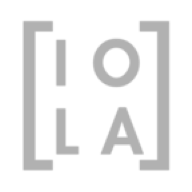
\includegraphics[height=2.2em]{images/iolalogo.png}}}
%	\lfoot{}
%	\renewcommand{\headrulewidth}{0pt}
%}
%
%\DeclareDocumentEnvironment{iola}{o}{%
%	\newpage
%	\pagestyle{iola}
%}{%
%	\newpage
%}


%%
% Allow hiding of environments
%%
\usepackage{environ}% http://ctan.org/pkg/environ
\makeatletter
\newcommand{\voidenvironment}[1]{%
  \expandafter\providecommand\csname env@#1@save@env\endcsname{}%
  \expandafter\providecommand\csname env@#1@process\endcsname{}%
  \@ifundefined{#1}{}{\RenewEnviron{#1}{}}%
}
\makeatother
% allow pagebreaks that only display in `standard` mode
\newcommand{\displayonlynewpage}{\begin{displayonly}\newpage\end{displayonly}}

%
% Set up the three render modes: standard, instructor, and solutions.
% These render with varying amounts of extra data (like solutions and notes)
%
\newtoggle{instructor}
\newtoggle{standard}
\newtoggle{solutions}
\newcommand{\setinstructor}{
	\toggletrue{instructor}
	\togglefalse{standard}
	\togglefalse{solutions}
}
\newcommand{\setstandard}{
	\togglefalse{instructor}
	\toggletrue{standard}
	\togglefalse{solutions}
}
\newcommand{\setsolutions}{
	\togglefalse{instructor}
	\togglefalse{standard}
	\toggletrue{solutions}
}

%
% Infer the document level from the \jobname
%
\usepackage{xstring}
\IfSubStr{\jobname}{\detokenize{solutions}}{\setsolutions}{
	\IfSubStr{\jobname}{\detokenize{instructor}}{\setinstructor}{
		\setstandard
	}
}

% Hide the non-problem environments
\newcommand{\coversubtitle}{}
\iftoggle{instructor}{
	\voidenvironment{displayonly}
	\renewcommand{\coversubtitle}{Instructor Guide}
}{}
\iftoggle{solutions}{
	\voidenvironment{displayonly}
	\voidenvironment{lesson}
	\voidenvironment{notes}
	\renewcommand{\coversubtitle}{Solutions}
}{}
\iftoggle{standard}{
	\voidenvironment{solution}
	\voidenvironment{annotation}
	\voidenvironment{lesson}
	\renewcommand{\coversubtitle}{MAT223 Notes}
}{}
%\voidenvironment{solution}
%\voidenvironment{annotation}
%\voidenvironment{lesson}
%%\voidenvironment{notes}
%%\voidenvironment{displayonly}


\begin{document}
\pagestyle{empty}


%\begin{tikzpicture}[remember picture,overlay, shift={(current page.north west)}, >=latex]
	%\definecolor{coverblue}{HTML}{ffd33c}
	\definecolor{coverblue}{HTML}{3FA2E4}
	\definecolor{coverpink}{HTML}{ff97e8}
	\definecolor{coveraccentpink}{HTML}{ffd33c}
	\definecolor{coverorange}{HTML}{ffffff}
	\definecolor{covershade}{HTML}{4D120D}
%	\definecolor{covershade}{HTML}{671811}

\newcommand{\modellingText}{(3.9498,32.8398) -- (9.8287,32.8398) -- (17.2701,52.6836) --
        (24.7506,32.8398) -- (30.6295,32.8398) -- (30.6295,62.0000) --
        (26.7818,62.0000) -- (26.7818,36.3945) -- (19.2623,56.3945) --
        (15.2974,56.3945) -- (7.7779,36.3945) -- (7.7779,62.0000) -- (3.9498,62.0000)
        -- cycle

		(46.8013,42.6445) .. controls (44.8743,42.6445) and
        (43.3508,43.3997) .. (42.2310,44.9102) .. controls (41.1112,46.4076) and
        (40.5513,48.4648) .. (40.5513,51.0820) .. controls (40.5513,53.6992) and
        (41.1047,55.7630) .. (42.2115,57.2734) .. controls (43.3313,58.7708) and
        (44.8612,59.5195) .. (46.8013,59.5195) .. controls (48.7154,59.5195) and
        (50.2323,58.7643) .. (51.3521,57.2539) .. controls (52.4719,55.7435) and
        (53.0318,53.6862) .. (53.0318,51.0820) .. controls (53.0318,48.4909) and
        (52.4719,46.4401) .. (51.3521,44.9297) .. controls (50.2323,43.4062) and
        (48.7154,42.6445) .. (46.8013,42.6445) -- cycle(46.8013,39.5977) .. controls
        (49.9263,39.5977) and (52.3808,40.6133) .. (54.1646,42.6445) .. controls
        (55.9485,44.6758) and (56.8404,47.4883) .. (56.8404,51.0820) .. controls
        (56.8404,54.6628) and (55.9485,57.4753) .. (54.1646,59.5195) .. controls
        (52.3808,61.5508) and (49.9263,62.5664) .. (46.8013,62.5664) .. controls
        (43.6633,62.5664) and (41.2024,61.5508) .. (39.4185,59.5195) .. controls
        (37.6477,57.4753) and (36.7623,54.6628) .. (36.7623,51.0820) .. controls
        (36.7623,47.4883) and (37.6477,44.6758) .. (39.4185,42.6445) .. controls
        (41.2024,40.6133) and (43.6633,39.5977) .. (46.8013,39.5977) -- cycle

		(77.1724,43.4453) -- (77.1724,31.6094) -- (80.7662,31.6094) --
        (80.7662,62.0000) -- (77.1724,62.0000) -- (77.1724,58.7188) .. controls
        (76.4172,60.0208) and (75.4602,60.9909) .. (74.3013,61.6289) .. controls
        (73.1555,62.2539) and (71.7753,62.5664) .. (70.1607,62.5664) .. controls
        (67.5175,62.5664) and (65.3625,61.5117) .. (63.6959,59.4023) .. controls
        (62.0422,57.2930) and (61.2154,54.5195) .. (61.2154,51.0820) .. controls
        (61.2154,47.6445) and (62.0422,44.8711) .. (63.6959,42.7617) .. controls
        (65.3625,40.6523) and (67.5175,39.5977) .. (70.1607,39.5977) .. controls
        (71.7753,39.5977) and (73.1555,39.9167) .. (74.3013,40.5547) .. controls
        (75.4602,41.1797) and (76.4172,42.1432) .. (77.1724,43.4453) --
        cycle(64.9263,51.0820) .. controls (64.9263,53.7253) and (65.4667,55.8021) ..
        (66.5474,57.3125) .. controls (67.6412,58.8099) and (69.1386,59.5586) ..
        (71.0396,59.5586) .. controls (72.9407,59.5586) and (74.4381,58.8099) ..
        (75.5318,57.3125) .. controls (76.6256,55.8021) and (77.1724,53.7253) ..
        (77.1724,51.0820) .. controls (77.1724,48.4388) and (76.6256,46.3685) ..
        (75.5318,44.8711) .. controls (74.4381,43.3607) and (72.9407,42.6055) ..
        (71.0396,42.6055) .. controls (69.1386,42.6055) and (67.6412,43.3607) ..
        (66.5474,44.8711) .. controls (65.4667,46.3685) and (64.9263,48.4388) ..
        (64.9263,51.0820) -- cycle

		(106.8795,50.1641) -- (106.8795,51.9219) -- (90.3560,51.9219)
        .. controls (90.5123,54.3958) and (91.2545,56.2839) .. (92.5826,57.5859) ..
        controls (93.9237,58.8750) and (95.7857,59.5195) .. (98.1685,59.5195) ..
        controls (99.5487,59.5195) and (100.8834,59.3503) .. (102.1724,59.0117) ..
        controls (103.4745,58.6732) and (104.7636,58.1654) .. (106.0396,57.4883) --
        (106.0396,60.8867) .. controls (104.7506,61.4336) and (103.4289,61.8503) ..
        (102.0748,62.1367) .. controls (100.7206,62.4232) and (99.3469,62.5664) ..
        (97.9537,62.5664) .. controls (94.4641,62.5664) and (91.6972,61.5508) ..
        (89.6529,59.5195) .. controls (87.6217,57.4883) and (86.6060,54.7409) ..
        (86.6060,51.2773) .. controls (86.6060,47.6966) and (87.5696,44.8581) ..
        (89.4967,42.7617) .. controls (91.4368,40.6523) and (94.0474,39.5977) ..
        (97.3287,39.5977) .. controls (100.2714,39.5977) and (102.5956,40.5482) ..
        (104.3013,42.4492) .. controls (106.0201,44.3372) and (106.8795,46.9089) ..
        (106.8795,50.1641) -- cycle(103.2857,49.1094) .. controls (103.2597,47.1432)
        and (102.7063,45.5742) .. (101.6256,44.4023) .. controls (100.5579,43.2305)
        and (99.1386,42.6445) .. (97.3677,42.6445) .. controls (95.3625,42.6445) and
        (93.7545,43.2109) .. (92.5435,44.3438) .. controls (91.3456,45.4766) and
        (90.6555,47.0716) .. (90.4732,49.1289) -- cycle

		(112.7779,31.6094) -- (116.3717,31.6094) -- (116.3717,62.0000)
        -- (112.7779,62.0000) -- cycle

		(123.8717,31.6094) -- (127.4654,31.6094) -- (127.4654,62.0000)
        -- (123.8717,62.0000) -- cycle

		(134.9654,40.1250) -- (138.5592,40.1250) -- (138.5592,62.0000)
        -- (134.9654,62.0000) -- cycle(134.9654,31.6094) -- (138.5592,31.6094) --
        (138.5592,36.1602) -- (134.9654,36.1602) -- cycle

		(164.2428,48.7969) -- (164.2428,62.0000) -- (160.6490,62.0000)
        -- (160.6490,48.9141) .. controls (160.6490,46.8438) and (160.2454,45.2943) ..
        (159.4381,44.2656) .. controls (158.6308,43.2370) and (157.4198,42.7227) ..
        (155.8053,42.7227) .. controls (153.8651,42.7227) and (152.3352,43.3411) ..
        (151.2154,44.5781) .. controls (150.0956,45.8151) and (149.5357,47.5013) ..
        (149.5357,49.6367) -- (149.5357,62.0000) -- (145.9224,62.0000) --
        (145.9224,40.1250) -- (149.5357,40.1250) -- (149.5357,43.5234) .. controls
        (150.3951,42.2083) and (151.4042,41.2253) .. (152.5631,40.5742) .. controls
        (153.7349,39.9232) and (155.0826,39.5977) .. (156.6060,39.5977) .. controls
        (159.1191,39.5977) and (161.0201,40.3789) .. (162.3092,41.9414) .. controls
        (163.5982,43.4909) and (164.2428,45.7760) .. (164.2428,48.7969) -- cycle

		(185.8443,50.8086) .. controls (185.8443,48.2044) and
        (185.3039,46.1862) .. (184.2232,44.7539) .. controls (183.1555,43.3216) and
        (181.6516,42.6055) .. (179.7115,42.6055) .. controls (177.7844,42.6055) and
        (176.2805,43.3216) .. (175.1998,44.7539) .. controls (174.1321,46.1862) and
        (173.5982,48.2044) .. (173.5982,50.8086) .. controls (173.5982,53.3997) and
        (174.1321,55.4115) .. (175.1998,56.8438) .. controls (176.2805,58.2760) and
        (177.7844,58.9922) .. (179.7115,58.9922) .. controls (181.6516,58.9922) and
        (183.1555,58.2760) .. (184.2232,56.8438) .. controls (185.3039,55.4115) and
        (185.8443,53.3997) .. (185.8443,50.8086) -- cycle(189.4381,59.2852) ..
        controls (189.4381,63.0091) and (188.6112,65.7760) .. (186.9576,67.5859) ..
        controls (185.3040,69.4089) and (182.7714,70.3203) .. (179.3599,70.3203) ..
        controls (178.0969,70.3203) and (176.9055,70.2227) .. (175.7857,70.0273) ..
        controls (174.6659,69.8451) and (173.5787,69.5586) .. (172.5240,69.1680) --
        (172.5240,65.6719) .. controls (173.5787,66.2448) and (174.6204,66.6680) ..
        (175.6490,66.9414) .. controls (176.6776,67.2148) and (177.7258,67.3516) ..
        (178.7935,67.3516) .. controls (181.1503,67.3516) and (182.9146,66.7331) ..
        (184.0865,65.4961) .. controls (185.2584,64.2721) and (185.8443,62.4167) ..
        (185.8443,59.9297) -- (185.8443,58.1523) .. controls (185.1021,59.4414) and
        (184.1516,60.4049) .. (182.9928,61.0430) .. controls (181.8339,61.6810) and
        (180.4472,62.0000) .. (178.8326,62.0000) .. controls (176.1503,62.0000) and
        (173.9888,60.9779) .. (172.3482,58.9336) .. controls (170.7076,56.8893) and
        (169.8873,54.1810) .. (169.8873,50.8086) .. controls (169.8873,47.4232) and
        (170.7076,44.7083) .. (172.3482,42.6641) .. controls (173.9888,40.6198) and
        (176.1503,39.5977) .. (178.8326,39.5977) .. controls (180.4472,39.5977) and
        (181.8339,39.9167) .. (182.9928,40.5547) .. controls (184.1516,41.1927) and
        (185.1021,42.1562) .. (185.8443,43.4453) -- (185.8443,40.1250) --
        (189.4381,40.1250) -- cycle}
        

\newcommand{\withDifferentialText}{(0.8638,51.0625) -- (2.6607,51.0625) -- (4.9068,59.5977) --
        (7.1431,51.0625) -- (9.2623,51.0625) -- (11.5084,59.5977) -- (13.7447,51.0625)
        -- (15.5416,51.0625) -- (12.6802,62.0000) -- (10.5611,62.0000) --
        (8.2076,53.0352) -- (5.8443,62.0000) -- (3.7252,62.0000) -- cycle
        
        (18.2760,51.0625) -- (20.0728,51.0625) -- (20.0728,62.0000) --
        (18.2760,62.0000) -- cycle(18.2760,46.8047) -- (20.0728,46.8047) --
        (20.0728,49.0801) -- (18.2760,49.0801) -- cycle
        
        (25.6002,47.9570) -- (25.6002,51.0625) -- (29.3013,51.0625) --
        (29.3013,52.4590) -- (25.6002,52.4590) -- (25.6002,58.3965) .. controls
        (25.6002,59.2884) and (25.7206,59.8613) .. (25.9615,60.1152) .. controls
        (26.2089,60.3691) and (26.7069,60.4961) .. (27.4556,60.4961) --
        (29.3013,60.4961) -- (29.3013,62.0000) -- (27.4556,62.0000) .. controls
        (26.0689,62.0000) and (25.1119,61.7428) .. (24.5845,61.2285) .. controls
        (24.0572,60.7077) and (23.7935,59.7637) .. (23.7935,58.3965) --
        (23.7935,52.4590) -- (22.4752,52.4590) -- (22.4752,51.0625) --
        (23.7935,51.0625) -- (23.7935,47.9570) -- cycle
        
        (40.7662,55.3984) -- (40.7662,62.0000) -- (38.9693,62.0000) --
        (38.9693,55.4570) .. controls (38.9693,54.4219) and (38.7675,53.6471) ..
        (38.3638,53.1328) .. controls (37.9602,52.6185) and (37.3547,52.3613) ..
        (36.5474,52.3613) .. controls (35.5774,52.3613) and (34.8124,52.6706) ..
        (34.2525,53.2891) .. controls (33.6926,53.9076) and (33.4127,54.7507) ..
        (33.4127,55.8184) -- (33.4127,62.0000) -- (31.6060,62.0000) --
        (31.6060,46.8047) -- (33.4127,46.8047) -- (33.4127,52.7617) .. controls
        (33.8424,52.1042) and (34.3469,51.6126) .. (34.9263,51.2871) .. controls
        (35.5123,50.9616) and (36.1861,50.7988) .. (36.9478,50.7988) .. controls
        (38.2043,50.7988) and (39.1549,51.1895) .. (39.7994,51.9707) .. controls
        (40.4439,52.7454) and (40.7662,53.8880) .. (40.7662,55.3984) -- cycle
        
        (52.7877,49.0410) -- (52.7877,60.3789) -- (55.1705,60.3789) ..
        controls (57.1822,60.3789) and (58.6536,59.9232) .. (59.5845,59.0117) ..
        controls (60.5220,58.1003) and (60.9908,56.6615) .. (60.9908,54.6953) ..
        controls (60.9908,52.7422) and (60.5220,51.3132) .. (59.5845,50.4082) ..
        controls (58.6536,49.4967) and (57.1822,49.0410) .. (55.1705,49.0410) --
        cycle(50.8150,47.4199) -- (54.8678,47.4199) .. controls (57.6933,47.4199) and
        (59.7668,48.0091) .. (61.0885,49.1875) .. controls (62.4101,50.3594) and
        (63.0709,52.1953) .. (63.0709,54.6953) .. controls (63.0709,57.2083) and
        (62.4068,59.0540) .. (61.0787,60.2324) .. controls (59.7506,61.4108) and
        (57.6803,62.0000) .. (54.8678,62.0000) -- (50.8150,62.0000) -- cycle
        
        (66.1275,51.0625) -- (67.9244,51.0625) -- (67.9244,62.0000) --
        (66.1275,62.0000) -- cycle(66.1275,46.8047) -- (67.9244,46.8047) --
        (67.9244,49.0801) -- (66.1275,49.0801) -- cycle
        
        (83.9498,46.8047) -- (83.9498,48.2988) -- (82.2310,48.2988) ..
        controls (81.5865,48.2988) and (81.1373,48.4290) .. (80.8834,48.6895) ..
        controls (80.6360,48.9499) and (80.5123,49.4186) .. (80.5123,50.0957) --
        (80.5123,51.0625) -- (83.4713,51.0625) -- (83.4713,52.4590) --
        (80.5123,52.4590) -- (80.5123,62.0000) -- (78.7056,62.0000) --
        (78.7056,52.4590) -- (73.7740,52.4590) -- (73.7740,62.0000) --
        (71.9674,62.0000) -- (71.9674,52.4590) -- (70.2486,52.4590) --
        (70.2486,51.0625) -- (71.9674,51.0625) -- (71.9674,50.3008) .. controls
        (71.9674,49.0833) and (72.2506,48.1979) .. (72.8170,47.6445) .. controls
        (73.3834,47.0846) and (74.2818,46.8047) .. (75.5123,46.8047) --
        (77.2115,46.8047) -- (77.2115,48.2988) -- (75.4928,48.2988) .. controls
        (74.8482,48.2988) and (74.3990,48.4290) .. (74.1451,48.6895) .. controls
        (73.8977,48.9499) and (73.7740,49.4186) .. (73.7740,50.0957) --
        (73.7740,51.0625) -- (78.7056,51.0625) -- (78.7056,50.3008) .. controls
        (78.7056,49.0833) and (78.9888,48.1979) .. (79.5553,47.6445) .. controls
        (80.1217,47.0846) and (81.0201,46.8047) .. (82.2506,46.8047) -- cycle
        
        (94.8189,56.0820) -- (94.8189,56.9609) -- (86.5572,56.9609) ..
        controls (86.6353,58.1979) and (87.0064,59.1419) .. (87.6705,59.7930) ..
        controls (88.3411,60.4375) and (89.2720,60.7598) .. (90.4635,60.7598) ..
        controls (91.1536,60.7598) and (91.8209,60.6751) .. (92.4654,60.5059) ..
        controls (93.1164,60.3366) and (93.7610,60.0827) .. (94.3990,59.7441) --
        (94.3990,61.4434) .. controls (93.7545,61.7168) and (93.0937,61.9251) ..
        (92.4166,62.0684) .. controls (91.7395,62.2116) and (91.0526,62.2832) ..
        (90.3560,62.2832) .. controls (88.6112,62.2832) and (87.2278,61.7754) ..
        (86.2056,60.7598) .. controls (85.1900,59.7441) and (84.6822,58.3704) ..
        (84.6822,56.6387) .. controls (84.6822,54.8483) and (85.1640,53.4290) ..
        (86.1275,52.3809) .. controls (87.0976,51.3262) and (88.4029,50.7988) ..
        (90.0435,50.7988) .. controls (91.5149,50.7988) and (92.6770,51.2741) ..
        (93.5299,52.2246) .. controls (94.3892,53.1686) and (94.8189,54.4544) ..
        (94.8189,56.0820) -- cycle(93.0220,55.5547) .. controls (93.0090,54.5716) and
        (92.7323,53.7871) .. (92.1920,53.2012) .. controls (91.6581,52.6152) and
        (90.9485,52.3223) .. (90.0631,52.3223) .. controls (89.0605,52.3223) and
        (88.2564,52.6055) .. (87.6510,53.1719) .. controls (87.0520,53.7383) and
        (86.7069,54.5358) .. (86.6158,55.5645) -- cycle
        
        (104.1060,52.7422) .. controls (103.9042,52.6250) and
        (103.6829,52.5404) .. (103.4420,52.4883) .. controls (103.2076,52.4297) and
        (102.9472,52.4004) .. (102.6607,52.4004) .. controls (101.6451,52.4004) and
        (100.8638,52.7324) .. (100.3170,53.3965) .. controls (99.7766,54.0540) and
        (99.5064,55.0013) .. (99.5064,56.2383) -- (99.5064,62.0000) --
        (97.6998,62.0000) -- (97.6998,51.0625) -- (99.5064,51.0625) --
        (99.5064,52.7617) .. controls (99.8840,52.0977) and (100.3756,51.6061) ..
        (100.9810,51.2871) .. controls (101.5865,50.9616) and (102.3222,50.7988) ..
        (103.1881,50.7988) .. controls (103.3118,50.7988) and (103.4485,50.8086) ..
        (103.5982,50.8281) .. controls (103.7480,50.8411) and (103.9140,50.8639) ..
        (104.0963,50.8965) -- cycle
        
        (114.9361,56.0820) -- (114.9361,56.9609) -- (106.6744,56.9609)
        .. controls (106.7525,58.1979) and (107.1236,59.1419) .. (107.7877,59.7930) ..
        controls (108.4582,60.4375) and (109.3892,60.7598) .. (110.5806,60.7598) ..
        controls (111.2707,60.7598) and (111.9381,60.6751) .. (112.5826,60.5059) ..
        controls (113.2336,60.3366) and (113.8782,60.0827) .. (114.5162,59.7441) --
        (114.5162,61.4434) .. controls (113.8717,61.7168) and (113.2108,61.9251) ..
        (112.5338,62.0684) .. controls (111.8567,62.2116) and (111.1698,62.2832) ..
        (110.4732,62.2832) .. controls (108.7284,62.2832) and (107.3450,61.7754) ..
        (106.3228,60.7598) .. controls (105.3072,59.7441) and (104.7994,58.3704) ..
        (104.7994,56.6387) .. controls (104.7994,54.8483) and (105.2812,53.4290) ..
        (106.2447,52.3809) .. controls (107.2148,51.3262) and (108.5201,50.7988) ..
        (110.1607,50.7988) .. controls (111.6321,50.7988) and (112.7942,51.2741) ..
        (113.6470,52.2246) .. controls (114.5064,53.1686) and (114.9361,54.4544) ..
        (114.9361,56.0820) -- cycle(113.1392,55.5547) .. controls (113.1262,54.5716)
        and (112.8495,53.7871) .. (112.3092,53.2012) .. controls (111.7753,52.6152)
        and (111.0657,52.3223) .. (110.1802,52.3223) .. controls (109.1776,52.3223)
        and (108.3736,52.6055) .. (107.7681,53.1719) .. controls (107.1692,53.7383)
        and (106.8241,54.5358) .. (106.7330,55.5645) -- cycle
        
        (126.9771,55.3984) -- (126.9771,62.0000) -- (125.1803,62.0000)
        -- (125.1803,55.4570) .. controls (125.1803,54.4219) and (124.9784,53.6471) ..
        (124.5748,53.1328) .. controls (124.1711,52.6185) and (123.5657,52.3613) ..
        (122.7584,52.3613) .. controls (121.7883,52.3613) and (121.0234,52.6706) ..
        (120.4635,53.2891) .. controls (119.9036,53.9076) and (119.6236,54.7507) ..
        (119.6236,55.8184) -- (119.6236,62.0000) -- (117.8170,62.0000) --
        (117.8170,51.0625) -- (119.6236,51.0625) -- (119.6236,52.7617) .. controls
        (120.0533,52.1042) and (120.5579,51.6126) .. (121.1373,51.2871) .. controls
        (121.7232,50.9616) and (122.3971,50.7988) .. (123.1588,50.7988) .. controls
        (124.4153,50.7988) and (125.3658,51.1895) .. (126.0103,51.9707) .. controls
        (126.6549,52.7454) and (126.9771,53.8880) .. (126.9771,55.3984) -- cycle
        
        (132.3580,47.9570) -- (132.3580,51.0625) -- (136.0592,51.0625)
        -- (136.0592,52.4590) -- (132.3580,52.4590) -- (132.3580,58.3965) .. controls
        (132.3580,59.2884) and (132.4784,59.8613) .. (132.7193,60.1152) .. controls
        (132.9667,60.3691) and (133.4648,60.4961) .. (134.2134,60.4961) --
        (136.0592,60.4961) -- (136.0592,62.0000) -- (134.2134,62.0000) .. controls
        (132.8267,62.0000) and (131.8697,61.7428) .. (131.3424,61.2285) .. controls
        (130.8150,60.7077) and (130.5513,59.7637) .. (130.5513,58.3965) --
        (130.5513,52.4590) -- (129.2330,52.4590) -- (129.2330,51.0625) --
        (130.5513,51.0625) -- (130.5513,47.9570) -- cycle
        
        (138.4322,51.0625) -- (140.2291,51.0625) -- (140.2291,62.0000)
        -- (138.4322,62.0000) -- cycle(138.4322,46.8047) -- (140.2291,46.8047) --
        (140.2291,49.0801) -- (138.4322,49.0801) -- cycle
        
        (148.9498,56.5020) .. controls (147.4980,56.5020) and
        (146.4921,56.6680) .. (145.9322,57.0000) .. controls (145.3723,57.3320) and
        (145.0924,57.8984) .. (145.0924,58.6992) .. controls (145.0924,59.3372) and
        (145.3007,59.8451) .. (145.7174,60.2227) .. controls (146.1405,60.5938) and
        (146.7135,60.7793) .. (147.4361,60.7793) .. controls (148.4322,60.7793) and
        (149.2297,60.4277) .. (149.8287,59.7246) .. controls (150.4342,59.0150) and
        (150.7369,58.0742) .. (150.7369,56.9023) -- (150.7369,56.5020) --
        cycle(152.5338,55.7598) -- (152.5338,62.0000) -- (150.7369,62.0000) --
        (150.7369,60.3398) .. controls (150.3267,61.0039) and (149.8157,61.4954) ..
        (149.2037,61.8145) .. controls (148.5917,62.1270) and (147.8430,62.2832) ..
        (146.9576,62.2832) .. controls (145.8378,62.2832) and (144.9459,61.9707) ..
        (144.2818,61.3457) .. controls (143.6243,60.7142) and (143.2955,59.8711) ..
        (143.2955,58.8164) .. controls (143.2955,57.5859) and (143.7056,56.6582) ..
        (144.5259,56.0332) .. controls (145.3528,55.4082) and (146.5832,55.0957) ..
        (148.2174,55.0957) -- (150.7369,55.0957) -- (150.7369,54.9199) .. controls
        (150.7369,54.0931) and (150.4635,53.4551) .. (149.9166,53.0059) .. controls
        (149.3762,52.5501) and (148.6145,52.3223) .. (147.6314,52.3223) .. controls
        (147.0064,52.3223) and (146.3977,52.3971) .. (145.8053,52.5469) .. controls
        (145.2128,52.6966) and (144.6431,52.9212) .. (144.0963,53.2207) --
        (144.0963,51.5605) .. controls (144.7538,51.3066) and (145.3918,51.1178) ..
        (146.0103,50.9941) .. controls (146.6288,50.8639) and (147.2310,50.7988) ..
        (147.8170,50.7988) .. controls (149.3990,50.7988) and (150.5806,51.2090) ..
        (151.3619,52.0293) .. controls (152.1431,52.8496) and (152.5338,54.0931) ..
        (152.5338,55.7598) -- cycle
        
        (156.2447,46.8047) -- (158.0416,46.8047) -- (158.0416,62.0000)
        -- (156.2447,62.0000) -- cycle}

\newcommand{\andDifferenceText}{(6.8795,56.5020) .. controls (5.4276,56.5020) and
        (4.4218,56.6680) .. (3.8619,57.0000) .. controls (3.3020,57.3320) and
        (3.0220,57.8984) .. (3.0220,58.6992) .. controls (3.0220,59.3372) and
        (3.2304,59.8451) .. (3.6470,60.2227) .. controls (4.0702,60.5938) and
        (4.6431,60.7793) .. (5.3658,60.7793) .. controls (6.3619,60.7793) and
        (7.1594,60.4277) .. (7.7584,59.7246) .. controls (8.3638,59.0150) and
        (8.6666,58.0742) .. (8.6666,56.9023) -- (8.6666,56.5020) --
        cycle(10.4635,55.7598) -- (10.4635,62.0000) -- (8.6666,62.0000) --
        (8.6666,60.3398) .. controls (8.2564,61.0039) and (7.7454,61.4954) ..
        (7.1334,61.8145) .. controls (6.5214,62.1270) and (5.7727,62.2832) ..
        (4.8873,62.2832) .. controls (3.7675,62.2832) and (2.8756,61.9707) ..
        (2.2115,61.3457) .. controls (1.5539,60.7142) and (1.2252,59.8711) ..
        (1.2252,58.8164) .. controls (1.2252,57.5859) and (1.6353,56.6582) ..
        (2.4556,56.0332) .. controls (3.2825,55.4082) and (4.5129,55.0957) ..
        (6.1470,55.0957) -- (8.6666,55.0957) -- (8.6666,54.9199) .. controls
        (8.6666,54.0931) and (8.3931,53.4551) .. (7.8463,53.0059) .. controls
        (7.3059,52.5501) and (6.5442,52.3223) .. (5.5611,52.3223) .. controls
        (4.9361,52.3223) and (4.3274,52.3971) .. (3.7349,52.5469) .. controls
        (3.1425,52.6966) and (2.5728,52.9212) .. (2.0260,53.2207) -- (2.0260,51.5605)
        .. controls (2.6835,51.3066) and (3.3215,51.1178) .. (3.9400,50.9941) ..
        controls (4.5585,50.8639) and (5.1607,50.7988) .. (5.7467,50.7988) .. controls
        (7.3287,50.7988) and (8.5103,51.2090) .. (9.2916,52.0293) .. controls
        (10.0728,52.8496) and (10.4635,54.0931) .. (10.4635,55.7598) -- cycle
        
        (23.2662,55.3984) -- (23.2662,62.0000) -- (21.4693,62.0000) --
        (21.4693,55.4570) .. controls (21.4693,54.4219) and (21.2675,53.6471) ..
        (20.8638,53.1328) .. controls (20.4602,52.6185) and (19.8547,52.3613) ..
        (19.0474,52.3613) .. controls (18.0774,52.3613) and (17.3124,52.6706) ..
        (16.7525,53.2891) .. controls (16.1926,53.9076) and (15.9127,54.7507) ..
        (15.9127,55.8184) -- (15.9127,62.0000) -- (14.1060,62.0000) --
        (14.1060,51.0625) -- (15.9127,51.0625) -- (15.9127,52.7617) .. controls
        (16.3424,52.1042) and (16.8469,51.6126) .. (17.4263,51.2871) .. controls
        (18.0123,50.9616) and (18.6861,50.7988) .. (19.4478,50.7988) .. controls
        (20.7043,50.7988) and (21.6549,51.1895) .. (22.2994,51.9707) .. controls
        (22.9439,52.7454) and (23.2662,53.8880) .. (23.2662,55.3984) -- cycle
        
        (34.0670,52.7227) -- (34.0670,46.8047) -- (35.8638,46.8047) --
        (35.8638,62.0000) -- (34.0670,62.0000) -- (34.0670,60.3594) .. controls
        (33.6894,61.0104) and (33.2108,61.4954) .. (32.6314,61.8145) .. controls
        (32.0585,62.1270) and (31.3684,62.2832) .. (30.5611,62.2832) .. controls
        (29.2395,62.2832) and (28.1620,61.7559) .. (27.3287,60.7012) .. controls
        (26.5019,59.6465) and (26.0885,58.2598) .. (26.0885,56.5410) .. controls
        (26.0885,54.8223) and (26.5019,53.4355) .. (27.3287,52.3809) .. controls
        (28.1620,51.3262) and (29.2395,50.7988) .. (30.5611,50.7988) .. controls
        (31.3684,50.7988) and (32.0585,50.9583) .. (32.6314,51.2773) .. controls
        (33.2108,51.5898) and (33.6894,52.0716) .. (34.0670,52.7227) --
        cycle(27.9439,56.5410) .. controls (27.9439,57.8626) and (28.2141,58.9010) ..
        (28.7545,59.6562) .. controls (29.3013,60.4049) and (30.0500,60.7793) ..
        (31.0006,60.7793) .. controls (31.9511,60.7793) and (32.6998,60.4049) ..
        (33.2467,59.6562) .. controls (33.7935,58.9010) and (34.0670,57.8626) ..
        (34.0670,56.5410) .. controls (34.0670,55.2194) and (33.7935,54.1842) ..
        (33.2467,53.4355) .. controls (32.6998,52.6803) and (31.9511,52.3027) ..
        (31.0006,52.3027) .. controls (30.0500,52.3027) and (29.3013,52.6803) ..
        (28.7545,53.4355) .. controls (28.2141,54.1842) and (27.9439,55.2194) ..
        (27.9439,56.5410) -- cycle
        
        (47.9830,49.0410) -- (47.9830,60.3789) -- (50.3658,60.3789) ..
        controls (52.3775,60.3789) and (53.8489,59.9232) .. (54.7799,59.0117) ..
        controls (55.7174,58.1003) and (56.1861,56.6615) .. (56.1861,54.6953) ..
        controls (56.1861,52.7422) and (55.7174,51.3132) .. (54.7799,50.4082) ..
        controls (53.8489,49.4967) and (52.3775,49.0410) .. (50.3658,49.0410) --
        cycle(46.0103,47.4199) -- (50.0631,47.4199) .. controls (52.8886,47.4199) and
        (54.9622,48.0091) .. (56.2838,49.1875) .. controls (57.6054,50.3594) and
        (58.2662,52.1953) .. (58.2662,54.6953) .. controls (58.2662,57.2083) and
        (57.6021,59.0540) .. (56.2740,60.2324) .. controls (54.9459,61.4108) and
        (52.8756,62.0000) .. (50.0631,62.0000) -- (46.0103,62.0000) -- cycle
        
        (61.3228,51.0625) -- (63.1197,51.0625) -- (63.1197,62.0000) --
        (61.3228,62.0000) -- cycle(61.3228,46.8047) -- (63.1197,46.8047) --
        (63.1197,49.0801) -- (61.3228,49.0801) -- cycle
        
        (79.1451,46.8047) -- (79.1451,48.2988) -- (77.4263,48.2988) ..
        controls (76.7818,48.2988) and (76.3326,48.4290) .. (76.0787,48.6895) ..
        controls (75.8313,48.9499) and (75.7076,49.4186) .. (75.7076,50.0957) --
        (75.7076,51.0625) -- (78.6666,51.0625) -- (78.6666,52.4590) --
        (75.7076,52.4590) -- (75.7076,62.0000) -- (73.9010,62.0000) --
        (73.9010,52.4590) -- (68.9693,52.4590) -- (68.9693,62.0000) --
        (67.1627,62.0000) -- (67.1627,52.4590) -- (65.4439,52.4590) --
        (65.4439,51.0625) -- (67.1627,51.0625) -- (67.1627,50.3008) .. controls
        (67.1627,49.0833) and (67.4459,48.1979) .. (68.0123,47.6445) .. controls
        (68.5787,47.0846) and (69.4771,46.8047) .. (70.7076,46.8047) --
        (72.4068,46.8047) -- (72.4068,48.2988) -- (70.6881,48.2988) .. controls
        (70.0435,48.2988) and (69.5943,48.4290) .. (69.3404,48.6895) .. controls
        (69.0930,48.9499) and (68.9693,49.4186) .. (68.9693,50.0957) --
        (68.9693,51.0625) -- (73.9010,51.0625) -- (73.9010,50.3008) .. controls
        (73.9010,49.0833) and (74.1842,48.1979) .. (74.7506,47.6445) .. controls
        (75.3170,47.0846) and (76.2154,46.8047) .. (77.4459,46.8047) -- cycle
        
        (90.0142,56.0820) -- (90.0142,56.9609) -- (81.7525,56.9609) ..
        controls (81.8306,58.1979) and (82.2017,59.1419) .. (82.8658,59.7930) ..
        controls (83.5364,60.4375) and (84.4674,60.7598) .. (85.6588,60.7598) ..
        controls (86.3489,60.7598) and (87.0162,60.6751) .. (87.6607,60.5059) ..
        controls (88.3118,60.3366) and (88.9563,60.0827) .. (89.5943,59.7441) --
        (89.5943,61.4434) .. controls (88.9498,61.7168) and (88.2890,61.9251) ..
        (87.6119,62.0684) .. controls (86.9348,62.2116) and (86.2480,62.2832) ..
        (85.5513,62.2832) .. controls (83.8066,62.2832) and (82.4231,61.7754) ..
        (81.4010,60.7598) .. controls (80.3853,59.7441) and (79.8775,58.3704) ..
        (79.8775,56.6387) .. controls (79.8775,54.8483) and (80.3593,53.4290) ..
        (81.3228,52.3809) .. controls (82.2929,51.3262) and (83.5982,50.7988) ..
        (85.2388,50.7988) .. controls (86.7102,50.7988) and (87.8723,51.2741) ..
        (88.7252,52.2246) .. controls (89.5845,53.1686) and (90.0142,54.4544) ..
        (90.0142,56.0820) -- cycle(88.2174,55.5547) .. controls (88.2043,54.5716) and
        (87.9276,53.7871) .. (87.3873,53.2012) .. controls (86.8534,52.6152) and
        (86.1438,52.3223) .. (85.2584,52.3223) .. controls (84.2558,52.3223) and
        (83.4517,52.6055) .. (82.8463,53.1719) .. controls (82.2473,53.7383) and
        (81.9023,54.5358) .. (81.8111,55.5645) -- cycle
        
        (99.3013,52.7422) .. controls (99.0995,52.6250) and
        (98.8782,52.5404) .. (98.6373,52.4883) .. controls (98.4029,52.4297) and
        (98.1425,52.4004) .. (97.8560,52.4004) .. controls (96.8404,52.4004) and
        (96.0592,52.7324) .. (95.5123,53.3965) .. controls (94.9719,54.0540) and
        (94.7017,55.0013) .. (94.7017,56.2383) -- (94.7017,62.0000) --
        (92.8951,62.0000) -- (92.8951,51.0625) -- (94.7017,51.0625) --
        (94.7017,52.7617) .. controls (95.0793,52.0977) and (95.5709,51.6061) ..
        (96.1763,51.2871) .. controls (96.7818,50.9616) and (97.5175,50.7988) ..
        (98.3834,50.7988) .. controls (98.5071,50.7988) and (98.6438,50.8086) ..
        (98.7935,50.8281) .. controls (98.9433,50.8411) and (99.1093,50.8639) ..
        (99.2916,50.8965) -- cycle
        
        (110.1314,56.0820) -- (110.1314,56.9609) -- (101.8697,56.9609)
        .. controls (101.9478,58.1979) and (102.3189,59.1419) .. (102.9830,59.7930) ..
        controls (103.6536,60.4375) and (104.5845,60.7598) .. (105.7760,60.7598) ..
        controls (106.4661,60.7598) and (107.1334,60.6751) .. (107.7779,60.5059) ..
        controls (108.4290,60.3366) and (109.0735,60.0827) .. (109.7115,59.7441) --
        (109.7115,61.4434) .. controls (109.0670,61.7168) and (108.4062,61.9251) ..
        (107.7291,62.0684) .. controls (107.0520,62.2116) and (106.3651,62.2832) ..
        (105.6685,62.2832) .. controls (103.9237,62.2832) and (102.5403,61.7754) ..
        (101.5181,60.7598) .. controls (100.5025,59.7441) and (99.9947,58.3704) ..
        (99.9947,56.6387) .. controls (99.9947,54.8483) and (100.4765,53.4290) ..
        (101.4400,52.3809) .. controls (102.4101,51.3262) and (103.7154,50.7988) ..
        (105.3560,50.7988) .. controls (106.8274,50.7988) and (107.9895,51.2741) ..
        (108.8424,52.2246) .. controls (109.7017,53.1686) and (110.1314,54.4544) ..
        (110.1314,56.0820) -- cycle(108.3346,55.5547) .. controls (108.3216,54.5716)
        and (108.0449,53.7871) .. (107.5045,53.2012) .. controls (106.9706,52.6152)
        and (106.2610,52.3223) .. (105.3756,52.3223) .. controls (104.3730,52.3223)
        and (103.5689,52.6055) .. (102.9635,53.1719) .. controls (102.3645,53.7383)
        and (102.0194,54.5358) .. (101.9283,55.5645) -- cycle
        
        (122.1724,55.3984) -- (122.1724,62.0000) -- (120.3756,62.0000)
        -- (120.3756,55.4570) .. controls (120.3756,54.4219) and (120.1737,53.6471) ..
        (119.7701,53.1328) .. controls (119.3665,52.6185) and (118.7610,52.3613) ..
        (117.9537,52.3613) .. controls (116.9836,52.3613) and (116.2187,52.6706) ..
        (115.6588,53.2891) .. controls (115.0989,53.9076) and (114.8189,54.7507) ..
        (114.8189,55.8184) -- (114.8189,62.0000) -- (113.0123,62.0000) --
        (113.0123,51.0625) -- (114.8189,51.0625) -- (114.8189,52.7617) .. controls
        (115.2486,52.1042) and (115.7532,51.6126) .. (116.3326,51.2871) .. controls
        (116.9185,50.9616) and (117.5924,50.7988) .. (118.3541,50.7988) .. controls
        (119.6106,50.7988) and (120.5611,51.1895) .. (121.2056,51.9707) .. controls
        (121.8502,52.7454) and (122.1724,53.8880) .. (122.1724,55.3984) -- cycle
        
        (133.6471,51.4824) -- (133.6471,53.1621) .. controls
        (133.1392,52.8822) and (132.6282,52.6738) .. (132.1138,52.5371) .. controls
        (131.6060,52.3939) and (131.0917,52.3223) .. (130.5709,52.3223) .. controls
        (129.4055,52.3223) and (128.5006,52.6934) .. (127.8560,53.4355) .. controls
        (127.2115,54.1712) and (126.8892,55.2064) .. (126.8892,56.5410) .. controls
        (126.8892,57.8757) and (127.2115,58.9141) .. (127.8560,59.6562) .. controls
        (128.5006,60.3919) and (129.4055,60.7598) .. (130.5709,60.7598) .. controls
        (131.0917,60.7598) and (131.6060,60.6914) .. (132.1138,60.5547) .. controls
        (132.6282,60.4115) and (133.1392,60.1999) .. (133.6471,59.9199) --
        (133.6471,61.5801) .. controls (133.1457,61.8145) and (132.6249,61.9902) ..
        (132.0846,62.1074) .. controls (131.5507,62.2246) and (130.9810,62.2832) ..
        (130.3756,62.2832) .. controls (128.7284,62.2832) and (127.4198,61.7656) ..
        (126.4498,60.7305) .. controls (125.4797,59.6953) and (124.9947,58.2988) ..
        (124.9947,56.5410) .. controls (124.9947,54.7572) and (125.4830,53.3542) ..
        (126.4596,52.3320) .. controls (127.4426,51.3099) and (128.7870,50.7988) ..
        (130.4928,50.7988) .. controls (131.0461,50.7988) and (131.5865,50.8574) ..
        (132.1138,50.9746) .. controls (132.6412,51.0853) and (133.1523,51.2546) ..
        (133.6471,51.4824) -- cycle
        
        (146.1471,56.0820) -- (146.1471,56.9609) -- (137.8853,56.9609)
        .. controls (137.9635,58.1979) and (138.3346,59.1419) .. (138.9986,59.7930) ..
        controls (139.6692,60.4375) and (140.6002,60.7598) .. (141.7916,60.7598) ..
        controls (142.4817,60.7598) and (143.1490,60.6751) .. (143.7935,60.5059) ..
        controls (144.4446,60.3366) and (145.0891,60.0827) .. (145.7271,59.7441) --
        (145.7271,61.4434) .. controls (145.0826,61.7168) and (144.4218,61.9251) ..
        (143.7447,62.0684) .. controls (143.0676,62.2116) and (142.3808,62.2832) ..
        (141.6842,62.2832) .. controls (139.9394,62.2832) and (138.5559,61.7754) ..
        (137.5338,60.7598) .. controls (136.5181,59.7441) and (136.0103,58.3704) ..
        (136.0103,56.6387) .. controls (136.0103,54.8483) and (136.4921,53.4290) ..
        (137.4556,52.3809) .. controls (138.4257,51.3262) and (139.7310,50.7988) ..
        (141.3717,50.7988) .. controls (142.8430,50.7988) and (144.0051,51.2741) ..
        (144.8580,52.2246) .. controls (145.7174,53.1686) and (146.1471,54.4544) ..
        (146.1471,56.0820) -- cycle(144.3502,55.5547) .. controls (144.3372,54.5716)
        and (144.0605,53.7871) .. (143.5201,53.2012) .. controls (142.9862,52.6152)
        and (142.2766,52.3223) .. (141.3912,52.3223) .. controls (140.3886,52.3223)
        and (139.5845,52.6055) .. (138.9791,53.1719) .. controls (138.3801,53.7383)
        and (138.0351,54.5358) .. (137.9439,55.5645) -- cycle}

\newcommand{\EquationsText}{(1.9869,47.4199) -- (11.2056,47.4199) -- (11.2056,49.0801) --
        (3.9595,49.0801) -- (3.9595,53.3965) -- (10.9029,53.3965) -- (10.9029,55.0566)
        -- (3.9595,55.0566) -- (3.9595,60.3398) -- (11.3814,60.3398) --
        (11.3814,62.0000) -- (1.9869,62.0000) -- cycle
        
        (15.6392,56.5410) .. controls (15.6392,57.8626) and
        (15.9094,58.9010) .. (16.4498,59.6562) .. controls (16.9967,60.4049) and
        (17.7454,60.7793) .. (18.6959,60.7793) .. controls (19.6464,60.7793) and
        (20.3951,60.4049) .. (20.9420,59.6562) .. controls (21.4888,58.9010) and
        (21.7623,57.8626) .. (21.7623,56.5410) .. controls (21.7623,55.2194) and
        (21.4888,54.1842) .. (20.9420,53.4355) .. controls (20.3951,52.6803) and
        (19.6464,52.3027) .. (18.6959,52.3027) .. controls (17.7454,52.3027) and
        (16.9967,52.6803) .. (16.4498,53.4355) .. controls (15.9094,54.1842) and
        (15.6392,55.2194) .. (15.6392,56.5410) -- cycle(21.7623,60.3594) .. controls
        (21.3847,61.0104) and (20.9062,61.4954) .. (20.3267,61.8145) .. controls
        (19.7538,62.1270) and (19.0637,62.2832) .. (18.2564,62.2832) .. controls
        (16.9348,62.2832) and (15.8573,61.7559) .. (15.0240,60.7012) .. controls
        (14.1972,59.6465) and (13.7838,58.2598) .. (13.7838,56.5410) .. controls
        (13.7838,54.8223) and (14.1972,53.4355) .. (15.0240,52.3809) .. controls
        (15.8573,51.3262) and (16.9348,50.7988) .. (18.2564,50.7988) .. controls
        (19.0637,50.7988) and (19.7538,50.9583) .. (20.3267,51.2773) .. controls
        (20.9062,51.5898) and (21.3847,52.0716) .. (21.7623,52.7227) --
        (21.7623,51.0625) -- (23.5592,51.0625) -- (23.5592,66.1602) --
        (21.7623,66.1602) -- cycle
        
        (27.0748,57.6836) -- (27.0748,51.0625) -- (28.8717,51.0625) --
        (28.8717,57.6152) .. controls (28.8717,58.6504) and (29.0735,59.4284) ..
        (29.4771,59.9492) .. controls (29.8808,60.4635) and (30.4862,60.7207) ..
        (31.2935,60.7207) .. controls (32.2636,60.7207) and (33.0286,60.4115) ..
        (33.5885,59.7930) .. controls (34.1549,59.1745) and (34.4381,58.3314) ..
        (34.4381,57.2637) -- (34.4381,51.0625) -- (36.2349,51.0625) --
        (36.2349,62.0000) -- (34.4381,62.0000) -- (34.4381,60.3203) .. controls
        (34.0019,60.9844) and (33.4941,61.4792) .. (32.9146,61.8047) .. controls
        (32.3417,62.1237) and (31.6744,62.2832) .. (30.9127,62.2832) .. controls
        (29.6562,62.2832) and (28.7024,61.8926) .. (28.0513,61.1113) .. controls
        (27.4003,60.3301) and (27.0748,59.1875) .. (27.0748,57.6836) --
        cycle(31.5963,50.7988) -- cycle
        
        (44.9263,56.5020) .. controls (43.4745,56.5020) and
        (42.4687,56.6680) .. (41.9088,57.0000) .. controls (41.3489,57.3320) and
        (41.0689,57.8984) .. (41.0689,58.6992) .. controls (41.0689,59.3372) and
        (41.2773,59.8451) .. (41.6939,60.2227) .. controls (42.1171,60.5938) and
        (42.6900,60.7793) .. (43.4127,60.7793) .. controls (44.4088,60.7793) and
        (45.2063,60.4277) .. (45.8053,59.7246) .. controls (46.4107,59.0150) and
        (46.7135,58.0742) .. (46.7135,56.9023) -- (46.7135,56.5020) --
        cycle(48.5103,55.7598) -- (48.5103,62.0000) -- (46.7135,62.0000) --
        (46.7135,60.3398) .. controls (46.3033,61.0039) and (45.7922,61.4954) ..
        (45.1803,61.8145) .. controls (44.5683,62.1270) and (43.8196,62.2832) ..
        (42.9342,62.2832) .. controls (41.8144,62.2832) and (40.9224,61.9707) ..
        (40.2584,61.3457) .. controls (39.6008,60.7142) and (39.2720,59.8711) ..
        (39.2720,58.8164) .. controls (39.2720,57.5859) and (39.6822,56.6582) ..
        (40.5025,56.0332) .. controls (41.3293,55.4082) and (42.5598,55.0957) ..
        (44.1939,55.0957) -- (46.7135,55.0957) -- (46.7135,54.9199) .. controls
        (46.7135,54.0931) and (46.4400,53.4551) .. (45.8931,53.0059) .. controls
        (45.3528,52.5501) and (44.5911,52.3223) .. (43.6080,52.3223) .. controls
        (42.9830,52.3223) and (42.3743,52.3971) .. (41.7818,52.5469) .. controls
        (41.1894,52.6966) and (40.6197,52.9212) .. (40.0728,53.2207) --
        (40.0728,51.5605) .. controls (40.7304,51.3066) and (41.3684,51.1178) ..
        (41.9869,50.9941) .. controls (42.6054,50.8639) and (43.2076,50.7988) ..
        (43.7935,50.7988) .. controls (45.3756,50.7988) and (46.5572,51.2090) ..
        (47.3385,52.0293) .. controls (48.1197,52.8496) and (48.5103,54.0931) ..
        (48.5103,55.7598) -- cycle
        
        (53.9986,47.9570) -- (53.9986,51.0625) -- (57.6998,51.0625) --
        (57.6998,52.4590) -- (53.9986,52.4590) -- (53.9986,58.3965) .. controls
        (53.9986,59.2884) and (54.1191,59.8613) .. (54.3599,60.1152) .. controls
        (54.6073,60.3691) and (55.1054,60.4961) .. (55.8541,60.4961) --
        (57.6998,60.4961) -- (57.6998,62.0000) -- (55.8541,62.0000) .. controls
        (54.4674,62.0000) and (53.5103,61.7428) .. (52.9830,61.2285) .. controls
        (52.4556,60.7077) and (52.1920,59.7637) .. (52.1920,58.3965) --
        (52.1920,52.4590) -- (50.8736,52.4590) -- (50.8736,51.0625) --
        (52.1920,51.0625) -- (52.1920,47.9570) -- cycle
        
        (60.0728,51.0625) -- (61.8697,51.0625) -- (61.8697,62.0000) --
        (60.0728,62.0000) -- cycle(60.0728,46.8047) -- (61.8697,46.8047) --
        (61.8697,49.0801) -- (60.0728,49.0801) -- cycle
        
        (69.8580,52.3223) .. controls (68.8944,52.3223) and
        (68.1327,52.6999) .. (67.5728,53.4551) .. controls (67.0129,54.2038) and
        (66.7330,55.2324) .. (66.7330,56.5410) .. controls (66.7330,57.8496) and
        (67.0097,58.8815) .. (67.5631,59.6367) .. controls (68.1230,60.3854) and
        (68.8879,60.7598) .. (69.8580,60.7598) .. controls (70.8150,60.7598) and
        (71.5735,60.3822) .. (72.1334,59.6270) .. controls (72.6933,58.8717) and
        (72.9732,57.8431) .. (72.9732,56.5410) .. controls (72.9732,55.2454) and
        (72.6933,54.2201) .. (72.1334,53.4648) .. controls (71.5735,52.7031) and
        (70.8150,52.3223) .. (69.8580,52.3223) -- cycle(69.8580,50.7988) .. controls
        (71.4205,50.7988) and (72.6477,51.3066) .. (73.5396,52.3223) .. controls
        (74.4316,53.3379) and (74.8775,54.7441) .. (74.8775,56.5410) .. controls
        (74.8775,58.3314) and (74.4316,59.7376) .. (73.5396,60.7598) .. controls
        (72.6477,61.7754) and (71.4205,62.2832) .. (69.8580,62.2832) .. controls
        (68.2890,62.2832) and (67.0585,61.7754) .. (66.1666,60.7598) .. controls
        (65.2812,59.7376) and (64.8385,58.3314) .. (64.8385,56.5410) .. controls
        (64.8385,54.7441) and (65.2812,53.3379) .. (66.1666,52.3223) .. controls
        (67.0585,51.3066) and (68.2890,50.7988) .. (69.8580,50.7988) -- cycle
        
        (86.9381,55.3984) -- (86.9381,62.0000) -- (85.1412,62.0000) --
        (85.1412,55.4570) .. controls (85.1412,54.4219) and (84.9394,53.6471) ..
        (84.5357,53.1328) .. controls (84.1321,52.6185) and (83.5266,52.3613) ..
        (82.7193,52.3613) .. controls (81.7493,52.3613) and (80.9843,52.6706) ..
        (80.4244,53.2891) .. controls (79.8645,53.9076) and (79.5845,54.7507) ..
        (79.5845,55.8184) -- (79.5845,62.0000) -- (77.7779,62.0000) --
        (77.7779,51.0625) -- (79.5845,51.0625) -- (79.5845,52.7617) .. controls
        (80.0142,52.1042) and (80.5188,51.6126) .. (81.0982,51.2871) .. controls
        (81.6842,50.9616) and (82.3580,50.7988) .. (83.1197,50.7988) .. controls
        (84.3762,50.7988) and (85.3267,51.1895) .. (85.9713,51.9707) .. controls
        (86.6158,52.7454) and (86.9381,53.8880) .. (86.9381,55.3984) -- cycle
        
        (97.5142,51.3848) -- (97.5142,53.0840) .. controls
        (97.0064,52.8236) and (96.4791,52.6283) .. (95.9322,52.4980) .. controls
        (95.3853,52.3678) and (94.8189,52.3027) .. (94.2330,52.3027) .. controls
        (93.3411,52.3027) and (92.6705,52.4395) .. (92.2213,52.7129) .. controls
        (91.7786,52.9863) and (91.5572,53.3965) .. (91.5572,53.9434) .. controls
        (91.5572,54.3600) and (91.7167,54.6888) .. (92.0357,54.9297) .. controls
        (92.3547,55.1641) and (92.9960,55.3887) .. (93.9595,55.6035) --
        (94.5748,55.7402) .. controls (95.8508,56.0137) and (96.7558,56.4010) ..
        (97.2896,56.9023) .. controls (97.8300,57.3971) and (98.1002,58.0905) ..
        (98.1002,58.9824) .. controls (98.1002,59.9980) and (97.6965,60.8021) ..
        (96.8892,61.3945) .. controls (96.0885,61.9870) and (94.9849,62.2832) ..
        (93.5787,62.2832) .. controls (92.9928,62.2832) and (92.3808,62.2246) ..
        (91.7428,62.1074) .. controls (91.1112,61.9967) and (90.4439,61.8275) ..
        (89.7408,61.5996) -- (89.7408,59.7441) .. controls (90.4049,60.0892) and
        (91.0592,60.3496) .. (91.7037,60.5254) .. controls (92.3482,60.6947) and
        (92.9862,60.7793) .. (93.6178,60.7793) .. controls (94.4641,60.7793) and
        (95.1151,60.6361) .. (95.5709,60.3496) .. controls (96.0266,60.0566) and
        (96.2545,59.6465) .. (96.2545,59.1191) .. controls (96.2545,58.6309) and
        (96.0885,58.2565) .. (95.7564,57.9961) .. controls (95.4309,57.7357) and
        (94.7115,57.4850) .. (93.5982,57.2441) -- (92.9732,57.0977) .. controls
        (91.8599,56.8633) and (91.0559,56.5052) .. (90.5611,56.0234) .. controls
        (90.0663,55.5352) and (89.8189,54.8678) .. (89.8189,54.0215) .. controls
        (89.8189,52.9928) and (90.1835,52.1986) .. (90.9127,51.6387) .. controls
        (91.6418,51.0788) and (92.6770,50.7988) .. (94.0181,50.7988) .. controls
        (94.6822,50.7988) and (95.3072,50.8477) .. (95.8931,50.9453) .. controls
        (96.4791,51.0430) and (97.0194,51.1895) .. (97.5142,51.3848) -- cycle}
        
	\begin{scope}
		\node[anchor=south east,inner sep=0pt,outer sep=0pt,] 
		at (current page.south east) {\includegraphics[width=\paperwidth, height=\paperheight]{images/MY-original.jpg}};

		\fill[path fading=north,covershade] (0,2.2in) rectangle ([yshift=-1.61in, xshift=2pt]current page.north east);
		\fill[covershade] (0,-1.5in) rectangle ([yshift=-2.7in]current page.north east);
		\fill[path fading=south, covershade] (0,-2.5in) rectangle ([xshift=1in,yshift=2in]current page.south east);
	\end{scope}


  \begin{scope}[yscale=-1, xscale=1, x=2.7pt, y=2.7pt,line join=miter,line cap=butt,line width=1.3pt, yshift=2.3cm, xshift=.7cm,
	  ]

	  \coordinate (E) at (57.55,23.15);
	  \coordinate (A) at (195.3,27.9);
	  \coordinate (C) at (195.3,104);
	  \coordinate (SUB) at (141, 10);
		
	  %\fill[coverblue, opacity=.7] \LINEARALGEBRAoutline;
	  %\draw[coverblue, line width=1.3pt] \LINEARALGEBRAoutline;

	\begin{scope}[shift={(0,-20)}]
	  \fill[coverblue, opacity=.55	] \modellingText;
	  \draw[coverblue, line width=1.3pt] \modellingText;
	\end{scope}

	\path[white] (SUB) node[anchor=north west] {\Large \bfseries \sffamily \coversubtitle};

	\begin{scope}[shift={(40,10)}]
	  \fill[coverblue, opacity=.45] \withDifferentialText;
	  \draw[coverblue, line width=1.3pt] \withDifferentialText;
	\end{scope}

	\begin{scope}[shift={(52,30)}]
	  \fill[coverblue, opacity=.35] \andDifferenceText;
	  \draw[coverblue, line width=1.3pt] \andDifferenceText;
	\end{scope}

	\begin{scope}[shift={(100,50)}]
	  \fill[coverblue, opacity=.25] \EquationsText;
	  \draw[coverblue, line width=1.3pt] \EquationsText;
	\end{scope}
	
	
	  
  \end{scope}


\newcommand{\authornames}{\huge \sffamily \bfseries \begin{tabular}{r}Bernardo Galv\~ao-Sousa\\Mihai Nica\\Jason Siefken\end{tabular}}
	\newcommand{\ypadd}{.5em}
	\newcommand{\xpadd}{1em}

	\draw (0, -24) node[right, xshift=10em] (AUTHOR) {\phantom{\authornames}};
	\path let \p1 = (AUTHOR.north) in coordinate (Ab1) at (0,\y1+\ypadd);
	\path let \p1 = (AUTHOR.north east) in coordinate (Ab2) at (\x1+\xpadd,\y1+\ypadd);
	\path let \p1 = (AUTHOR.south east) in coordinate (Ab3) at (\x1+\xpadd,\y1-\ypadd);
	\path let \p1 = (AUTHOR.south) in coordinate (Ab4) at (0,\y1-\ypadd);

	\path[fill=covershade, path fading=west, opacity=.8] (Ab1) -- (Ab2) -- (Ab3) -- (Ab4);
	\draw[covershade!80!black, line width=1.3pt] (Ab1) -- (Ab2) -- (Ab3) -- (Ab4);
	\draw (0, -24) node[right, xshift=10em, white] (AUTHOR) {\authornames};

\end{tikzpicture}

\newpage

\begin{center}
{\huge\bf Inquiry Based Modelling with Differential and Difference Equations}\\

\vspace{.7in}
{
\it \copyright\,Galvao-Sousa-Nica-Siefken, 2019--2020 \\
Creative Commons By-Attribution Share-Alike\, \makebox(30,5){
\includegraphics[height=1.2em]{by-sa.pdf}}
}
\end{center}

\section*{About the Document}


This document is a mix of student resources, student projects, problem sets, and labs. 
A typical class day looks like:
\begin{enumerate}
	\item \textbf{Preparation by students.} Students prepare for lecture by watching a short video and solving a short quiz. 

	\item \textbf{Introduction by instructor.} This may involve giving a broader context for the day's topics, or answering questions.

	\item \textbf{Students work on problems.} Students work individually or in small groups
		on the prescribed problem. During this time the instructor moves
		around the room addressing questions that students may have and giving
		one-on-one coaching.

	\item \textbf{Instructor intervention.} If most students have successfully solved
		the problem, the instructor regroups the class by providing a concise
		explanation so that everyone is ready to move to the next concept.
		This is also time for the instructor to ensure that everyone has
		understood the main point of the exercise (since it is sometimes
		easy to do some computation while being oblivious to the larger context).

		If students are having trouble, the instructor can give hints to
		the group, and additional guidance to ensure the students don't get
		frustrated to the point of giving up.

	\item \textbf{Repeat step 2.}
\end{enumerate}

Using this format, students are working (and happily so) most of the class. Further,
they are especially primed to hear the insights of the instructor, having already
invested substantially into each problem.

This problem-set is geared towards concepts instead of computation, though some problems
focus on simple computation.

\begin{annotation}
	\begin{goals}
	\Goal{http://creativecommons.org/\\licenses/by-sa/4.0/}

	\hfill \qrcode{http://creativecommons.org/licenses/by-sa/4.0/}	
	\end{goals}
\end{annotation}

{\bf License} Unless otherwise mentioned, pages of this document are licensed under
the Creative Commons By-Attribution Share-Alike License. That means, you are free
to use, copy, and modify this document provided that you provide attribution to the
previous copyright holders and you release your derivative work under the same license.
Full text of the license is at \url{http://creativecommons.org/licenses/by-sa/4.0/}

\begin{annotation}
	\begin{goals}
	\Goal{https://github.com/bigfatbernie/\\IBLmodellingDEs}
	
	\hfill \qrcode{https://github.com/bigfatbernie/IBLmodellingDEs}	
	\end{goals}
\end{annotation}

If you modify this document, you may add your name to the copyright list. Also,
if you think your contributions would be helpful to others, consider making a
pull request, or opening an \emph{issue} at \url{https://github.com/bigfatbernie/IBLmodellingDEs}

Content from other sources is reproduced here with permission and retains the
Author's copyright. Please see the footnote of each page to verify the
copyright.

\newpage

\tableofcontents

	
\newpage
\pagestyle{siefken}



%\addcontentsline{toc}{chapter}{Lessons}







\setcounter{page}{1}



%%%%%%%%%%%%%%%%%%%%%%%%%%%%%%%%%%%%%%%%%%%%%%%%%%%%%%%%%%%%%%%%%%%%%%%%
%
%		Chapter 1 - Mathematical Modelling
%
%%%%%%%%%%%%%%%%%%%%%%%%%%%%%%%%%%%%%%%%%%%%%%%%%%%%%%%%%%%%%%%%%%%%%%%%


\begin{topic}[Mathematical Modelling]
%\Title{Mathematical Modelling}


In this section, we study some strategies to model problems mathematically in an effective manner.



\end{topic}


\begin{lesson}
	\Title{Defining Problem Statement}

	\Heading{Objectives}
	\begin{itemize}
		\item The first step in Mathematical modelling is to define the problem
		\item A good way to do this is to figure out what is the ``mathematical object'' we are looking for at the end of the process

		\item The second step is to create a mind map of the problem. This is a structured way to brainstorm possible solutions and their requirements.
	\end{itemize}
	
	\Heading{Motivation} 

\begin{annotation}
	\begin{goals}
	\Goal{Extra Reading}
	Math Modelling: Getting started and getting solutions, Bliss-Fowler-Galluzzo
	
	\hfill \qrcode{https://m3challenge.siam.org/resources/modeling-handbook}	
	\end{goals}
\end{annotation}
	\Heading{Extra Reading} \href{https://m3challenge.siam.org/resources/modeling-handbook}{Math Modelling: Getting started and getting solutions, Bliss-Fowler-Galluzzo}

\end{lesson}




\section*{Step A. Defining the problem}
\addcontentsline{toc}{subsection}{Step A. Defining the problem}

The first step is to define the problem we want to solve or improve.

To do this, we should start from the end! We need to decide on what kind of mathematical object we will use in the end to show that we solved, or at least improved, the problem we were tasked with. \\


Once this is done, we can define the problem mathematically. 

\begin{example}
	Your team was tasked with optimizing the layout of an airport.
	
	You decided that in the end, to show that the team did find a good layout fo an airport, they will show
	\begin{itemize}
		\item $T = $ the total time (in minutes) necessary by the average person to walk from their airport transportation (taxi, train, bus) to their gate.
	\end{itemize}
	
	Once this decision is made, the problem to solve (or improve) becomes the following:
	
	\begin{itemize}
		\item Minimize $T$
	\end{itemize}

	There will probably be some constraints, which will be studied in Step C.

\end{example}


\vfill


\section*{Task 1.A: Elevator problem at theBigCompany}
\addcontentsline{toc}{subsection}{Task 1.A: Elevator problem at theBigCompany}


\begin{annotation}
	\begin{goals}
		\Goal{Make the question precise, bring it into a ``mathematical form''.}
		\begin{itemize}
			\item Choose a mathematical object best suited for the problem, e.g. a number, a geometric form, a graph, a function, an algorithm, ...

		\end{itemize}
	\end{goals}
%	\begin{notes}
%		
%		\begin{itemize}
%			\item There are many ways to solve this problem.
%				Some students
%				might start with equations. After they use their
%				equations to solve the problem, make them draw a picture
%				and come up with a graphical solution.
%
%			\item When the students start coming up with vector equations,
%				give them the vocabulary of \emph{linear
%				combinations}
%				and \emph{column vector notation}.
%		\end{itemize}
%	\end{notes}
\end{annotation}


You are hired by theBigCompany to help with their ``elevator problem''.

This is the email you received:

\begin{center}
	\color{blue}
	\begin{tabular}{?l}
	\begin{minipage}{.75\textwidth}
	-------- Forwarded Message -------- \\[10pt]
	\textcolor{black}{Date: } Mon, 16 September 2019 21:41:35 + 0000  \\
	\textcolor{black}{From: } CEO <theCEO@theBigCompany.ca> \\
	\textcolor{black}{To: } Human Resources <hr@theBigCompany.ca> \\
	\textcolor{black}{Subject: } they're still late !?\@\&! \\
	
	Hey Shophika! \\
	
	I still get complaints about staff being late, some by 15 minutes.
	
	With the staff we have, that's about one salary lost.
	
	Again the bottleneck of the elevators seems to be the problem.
	
	Can you suggest solutions? \\
	
	Thanks, the CEO
	\end{minipage}
	\end{tabular}
\end{center}


\vspace{5mm}

\begin{annotation}
	\begin{notes}
		
		\begin{itemize}
			\item Students will start discussing how to solve the problem
			\item This question deals with what will happen \textbf{after} solving the problem
			\item The goal of this question is to think about how to best tell a ``mathematically-challenged'' CEO that you solved the problem
		\end{itemize}
	\end{notes}
\end{annotation}

\paragraph{Scenario 1:}

With your team, you must decide on one answer and be prepared to report on your decision and the reason for your choice.

\subparagraph{Task.} What mathematical object would you use to convince the CEO that you have solved or improved the problem?








\newpage



\question
\label{object}
For each part, what ``mathematical object'' would you use to communicate that you have solved or improved the problem? Then define the problem mathematically.
\begin{parts}
	\item Help the city of Toronto choose the best recycling centre.
	\item Help the Canadian Institute of Health Information (CIHI) estimate how significant the outbreak of illnesses will be in the coming year in Canada.
	\item Create a mathematical model to rank roller coasters according to thrill factor.
	\item Gas stations offer different prices for gas. I would like to create an app that finds the best gas station to go to. What should ``best'' mean?
	\item The mayor of Toronto wants to extend the subway line with a new \textcolor{RoyalBlue}{blue line} as in Figure \ref{TTC}. Is it optimal?
	
	\item Is it better to buy or rent? 
	\begin{enumerate}
		\item Is it better to buy a car or rent Zipcar, Enterprise Carshare, or Car2go?
		\item Does the criteria you used to evaluate the previous question change if the question is whether to buy a bicycle or use Bike Share Toronto? 
	\end{enumerate}

	\begin{center}
	\begin{figure}[!htbp]
	\includegraphics*[width=500pt]{images/TTC-extension.png}
	\caption{Extension plans for Toronto subway line.}
	\label{TTC}	
	\end{figure}
	\end{center}
	
\end{parts}








\newpage

\section*{Step B. Building a mind map}
\addcontentsline{toc}{subsection}{Step B. Building a mind map}

\begin{annotation}
	\begin{notes}
	\begin{itemize}
		\item Students usually come up with more complicated variations:
		\begin{itemize}
			\item Money spent on late employees' salaries
			\item sum of time in minutes that employees are late counting only employees that are at most 15 minutes late
		\end{itemize}
		\item Stick with $R$, a simple first approach
	\end{itemize}	
	\end{notes}
	
\end{annotation}


A mind map is a tool to visually outline and organize ideas. Typically a key idea is the centre of a mind map and associated ideas are added to create a diagram that shows the flow of ideas. In Figure \ref{mindmap1}, we focus on the definition of ``best'', with three possible definitions
branching off to be further explored. From here, we can focus our attention on one of the three branches
at a time.

\begin{figure}[!htbp]
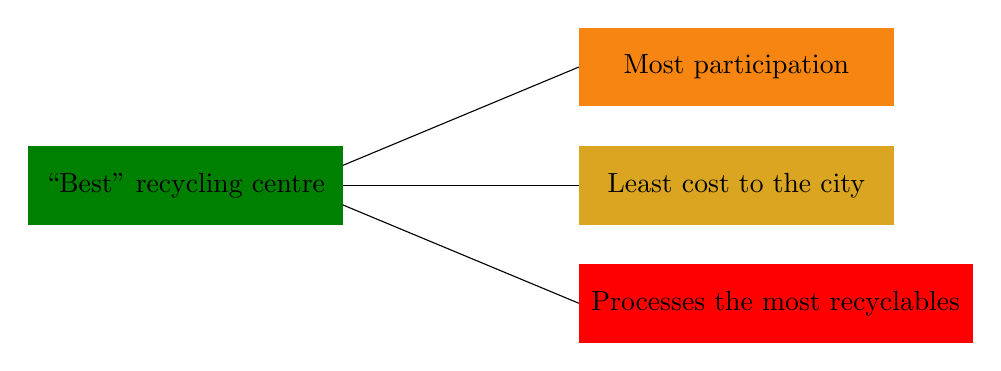
\begin{tikzpicture}
	\fill[color=Green] (0,0) rectangle (4,1) node[pos=.5] {\color{black}``Best'' recycling centre};
	\fill[color=BurntOrange] (7,2.5) rectangle (11,1.5) node[pos=.5] {\color{black}Most participation};
	\fill[color=Goldenrod] (7,0) rectangle (11,1) node[pos=.5] {\color{black}Least cost to the city};
	\fill[color=red] (7,-1.5) rectangle (12,-0.5) node[pos=.5] {\color{black}Processes the most recyclables};
	\draw (4,0.75) -- (7,2);
	\draw (4,0.5) -- (7,0.5);
	\draw (4,0.25) -- (7,-1);
\end{tikzpicture}
\caption{An example of a simple mind map.}
\label{mindmap1}
\end{figure}


Let's think about the least-cost option first. We probably can't determine how much any recycling program costs without knowing more about the recycling program, so a good place to start is to ask the question ``What kinds of recycling programs exist?''
If we aren't familiar with different types of recycling, we might need to do some research to see what kinds of programs exist.


A possible next step on your mind map for the least-cost approach could be the one shown in Figure \ref{mindmap2}.

\begin{figure}[!htbp]
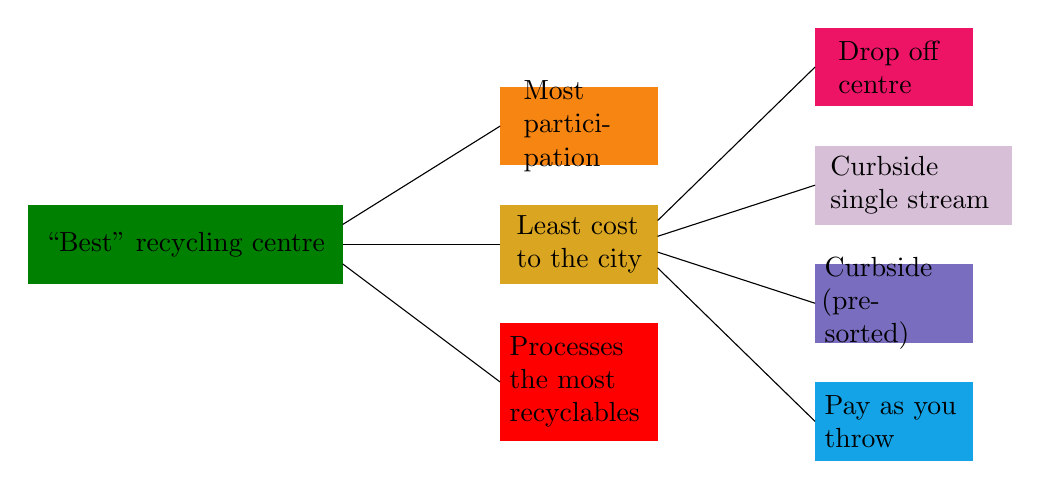
\begin{tikzpicture}
	\fill[color=Green] (0,0) rectangle (4,1) node[pos=.5] {\color{black}``Best'' recycling centre};
	\fill[color=BurntOrange] (6,2.5) rectangle (8,1.5) node[pos=.5] {\color{black}\begin{minipage}{40pt}\raggedright Most participation\end{minipage}};
	\fill[color=Goldenrod] (6,0) rectangle (8,1) node[pos=.5] {\color{black}\begin{minipage}{45pt}\raggedright Least cost to the city\end{minipage}};
	\fill[color=red] (6,-2) rectangle (8,-0.5) node[pos=.5] {\color{black}\begin{minipage}{50pt}\raggedright Processes the most recyclables\end{minipage}};
	\draw (4,0.75) -- (6,2);
	\draw (4,0.5) -- (6,0.5);
	\draw (4,0.25) -- (6,-1.25);
	\fill[color=WildStrawberry] (10,2.25) rectangle (12,3.25) node[pos=.5] {\color{black}\begin{minipage}{40pt}\raggedright Drop off centre\end{minipage}};	
	\fill[color=Thistle] (10,0.75) rectangle (12.5,1.75) node[pos=.5] {\color{black}\begin{minipage}{60pt}\raggedright Curbside single stream\end{minipage}};	
	\fill[color=Periwinkle] (10,0.25) rectangle (12,-0.75) node[pos=.5] {\color{black}\begin{minipage}{50pt}\raggedright Curbside (pre-sorted)\end{minipage}};	
	\fill[color=Cerulean] (10,-2.25) rectangle (12,-1.25) node[pos=.5] {\color{black}\begin{minipage}{50pt}\raggedright Pay as you throw\end{minipage}};
	\draw (8,0.8) -- (10,2.75);	
	\draw (8,0.6) -- (10,1.25);	
	\draw (8,0.4) -- (10,-0.25);	
	\draw (8,0.2) -- (10,-1.75);	
\end{tikzpicture}
\caption{Next step of a mind map.}
\label{mindmap2}
\end{figure}



\begin{annotation}
	\begin{goals}
		\Goal{FreeMind}

		\hfill \qrcode{http://freemind.sourceforge.net}	
	\end{goals}
\end{annotation}


\subparagraph{Software.} There is free online software to help creating a mind map. One such is \textcolor{blue}{\underline{\href{http://freemind.sourceforge.net}{FreeMind}}}.






\newpage

\section*{Task 1.B: Elevator problem at theBigCompany}
\addcontentsline{toc}{subsection}{Task 1.B: Elevator problem at theBigCompany}


\paragraph{Scenario 2:} \label{elevatorR}

Your team decides that the mathematical object you will use to show the CEO that you solved or improved the problem is
\begin{itemize}
	\item $R=$ the sum in minutes by which every employee is late.
\end{itemize}

Employees that are on time count for 0 minutes. 

\subparagraph{Task.} Create a mind map for the question: \quad How can $R$ be minimized?


\vfill

\question

For each part, create a mind map. Focus on the same approach you had for question \ref{object}.
\begin{parts}
	\item Help the city of Toronto choose the best recycling centre.
	\item Help the Canadian Institute of Health Information (CIHI) estimate how significant the outbreak of illnesses will be in the coming year in Canada.
	\item Create a mathematical model to rank roller coasters according to thrill factor.
	\item Gas stations offer different prices for gas. I would like to create an app that finds the best gas station to go to. What should ``best'' mean?
	\item The mayor of Toronto wants to extend the subway line with a new blue line as in Figure \ref{TTC}. Is it optimal?
	
	\item Is it better to buy a car or rent Zipcar, Enterprise Carshare, or Car2go?

	
\end{parts}








\begin{lesson}
	\Title{Making Assumptions}
	
	\Heading{Objectives}
	\begin{itemize}
		\item Bla bla bla	
	\end{itemize}
	
	\Heading{Motivation} 


\begin{annotation}
	\begin{goals}
	\Goal{Extra Reading}
	Math Modelling: Getting started and getting solutions, Bliss-Fowler-Galluzzo
	
	\hfill \qrcode{https://m3challenge.siam.org/resources/modeling-handbook}	
	\end{goals}
\end{annotation}
	\Heading{Extra Reading} \href{https://m3challenge.siam.org/resources/modeling-handbook}{Math Modelling: Getting started and getting solutions, Bliss-Fowler-Galluzzo}


\end{lesson}


\begin{annotation}
	\begin{notes}
		This is horrible and definitely needs to be worked on!
	\end{notes}
\end{annotation}









\section*{Step C. Making Assumptions}
\addcontentsline{toc}{subsection}{Step C. Making Assumptions}











\begin{lesson}
	\Title{Defining Variables}
	
	\Heading{Objectives}
	\begin{itemize}
		\item Bla bla bla	
	\end{itemize}
	
	\Heading{Motivation} 

\begin{annotation}
	\begin{goals}
	\Goal{Extra Reading}
	Math Modelling: Getting started and getting solutions, Bliss-Fowler-Galluzzo
	
	\hfill \qrcode{https://m3challenge.siam.org/resources/modeling-handbook}	
	\end{goals}
\end{annotation}
	\Heading{Extra Reading} \href{https://m3challenge.siam.org/resources/modeling-handbook}{Math Modelling: Getting started and getting solutions, Bliss-Fowler-Galluzzo}


\end{lesson}





\section*{Step D. Parameters or Variables?}
\addcontentsline{toc}{subsection}{Step D. Parameters or Variables?}


%There is a clear difference between \emph{variables} and \emph{parameters}. 

\begin{definition}[Variables and Parameters]

A \emph{variable} represents a model state, and may change during simulation.

A \emph{parameter} is commonly used to describe objects statically. A \emph{parameter} is normally a constant in a single simulation, and is changed only when you need to adjust your model behaviour. 
\end{definition}

%Use a variable instead of a parameter if you need to model some data unit continuously changing over time. Use a parameter instead of a variable if you just need to model some parameter of an object changed only at particular moments of time.



\begin{annotation}
	\begin{goals}
	\qrcode{https://en.wikipedia.org/wiki/Parameter\#Mathematical\_models}	
	\end{goals}
\end{annotation}
\begin{note}{(from Wikipedia)}
The quantities appearing in the equations we classify into variables and parameters. The distinction between these is not always clear cut, and it frequently depends on the context in which the variables appear. 

Usually a model is designed to explain the relationships that exist among quantities which can be measured independently in an experiment; these are the \emph{variables} of the model. 

To formulate these relationships, however, one frequently introduces ``constants'' which stand for inherent properties of nature (or of the materials and equipment used in a given experiment). These are the \emph{parameters}.	
\end{note}









The choice of question in the previous lesson should determine the \emph{dependent} variable.

%
%The \emph{parameters} are the independent variables in the problem, e.g. the speed of the elevators. The final answer will depend on the parameters in the problem. 
%
%We can estimate the parameters, and sometimes even change them. \\
%
%The \emph{variables} are dependent. This meant that if we change the parameters, the variables will change automatically. 




\vfill





\section*{Task 1.D: Elevator problem at theBigCompany}
\addcontentsline{toc}{subsection}{Task 1.D: Elevator problem at theBigCompany}


We now give you some technical details about theBigCompany:

\begin{itemize}
	\item The company occupies the floors 30--33 of the building Place Ville-Marie (in Montr\'eal).
	\item Personnel is distributed in the following way: 
	\begin{itemize}
		\item 350 employees in floor 30,
		\item 350 employees in floor 31,
		\item 250 employees in floor 32, 
		\item 150 employees in floor 33.
	\end{itemize}
\end{itemize}

\textsl{Note.} Even though these details are fictional, the numbers respect the building code.


\subparagraph{Tasks.} Focus on a \textbf{few} parameters and variables. State hypotheses.

\begin{enumerate} 

	\item With your team, decide on what kind of information you would need to have to be able to solve this problem.

	\item Find the relevant information about the elevators (search the internet, by experimentation). Check the reliability of the data you found.

	\item For the relevant information that you cannot obtain, make assumptions. These assumptions should be reasonable and you should be able to justify them.
\end{enumerate}

\vspace{0.5in}

\newpage
%\vfill



\question
For each part, you are required to make an estimate for some quantity. Make assumptions and justify them in order to solve the problem.
\begin{parts}
	\item What is the number of piano players in Toronto? \hfill \emph{(Fermi problem)}
	\item How many linear km of roads are there in Toronto?
	\item How much salt the city of Toronto needs for its roads during the Winter?
	\item The skating season in Canada is shortening: What are the key-factors determining its length?
	
\end{parts}








\begin{lesson}
	\Title{Building Solutions}
	
	\Heading{Objectives}
	\begin{itemize}
		\item Bla bla bla	
	\end{itemize}
	
	\Heading{Motivation} 

\begin{annotation}
	\begin{goals}
	\Goal{Extra Reading}
	Math Modelling: Getting started and getting solutions, Bliss-Fowler-Galluzzo
	
	\hfill \qrcode{https://m3challenge.siam.org/resources/modeling-handbook}	
	\end{goals}
\end{annotation}
	\Heading{Extra Reading} \href{https://m3challenge.siam.org/resources/modeling-handbook}{Math Modelling: Getting started and getting solutions, Bliss-Fowler-Galluzzo}
\end{lesson}







\begin{lesson}
	\Title{Model Assessment}
	
	\Heading{Objectives}
	\begin{itemize}
		\item Bla bla bla	
	\end{itemize}
	
	\Heading{Motivation} 

\begin{annotation}
	\begin{goals}
	\Goal{Extra Reading}
	Math Modelling: Getting started and getting solutions, Bliss-Fowler-Galluzzo
	
	\hfill \qrcode{https://m3challenge.siam.org/resources/modeling-handbook}	
	\end{goals}
\end{annotation}
	\Heading{Extra Reading} \href{https://m3challenge.siam.org/resources/modeling-handbook}{Math Modelling: Getting started and getting solutions, Bliss-Fowler-Galluzzo}

\end{lesson}





\begin{lesson}
	\Title{Putting it all together}
	\Heading{Textbook} \href{https://m3challenge.siam.org/resources/modeling-handbook}{Math Modelling: Getting started and getting solutions, Bliss-Fowler-Galluzzo}
	
	\Heading{Objectives}
	\begin{itemize}
		\item Bla bla bla	
	\end{itemize}
	
	\Heading{Motivation} 


\end{lesson}

%%%%%%%%%%%%%%%%%%%%%%%%%%%%%%%%%%%%%%%%%%%%%%%%%%%%%%%%%%%%%%%%%%%%%%%%
%
%		Chapter 2 - First-order Models
%
%%%%%%%%%%%%%%%%%%%%%%%%%%%%%%%%%%%%%%%%%%%%%%%%%%%%%%%%%%%%%%%%%%%%%%%%


\begin{topic}[First-Order Models]

\end{topic}




%%%%%%%%%%%%%%%%%%%%%%%%%%%%%%%%%%%%%%%%%%%%%%%%%%%%%%%%%%%%%%%%%%%%%%%%
%		Basic Models


\begin{lesson}
	\Title{Basic Models}
	\Heading{Textbook}	
	\Heading{Objectives}
	\begin{itemize}
		\item Bla bla bla	
	\end{itemize}
	
	\Heading{Motivation} 


\end{lesson}






%%%%%%%%%%%%%%%%%%%%%%%%%%%%%%%%%%%%%%%%%%%%%%%%%%%%%%%%%%%%%%%%%%%%%%%%
%		Direction Fields


\begin{lesson}
	\Title{Direction Fields}	
	\Heading{Objectives}
	\begin{itemize}
		\item Bla bla bla	
	\end{itemize}
	
	\Heading{Motivation} 


\end{lesson}



















%%%%%%%%%%%%%%%%%%%%%%%%%%%%%%%%%%%%%%%%%%%%%%%%%%%%%%%%%%%%%%%%%%%%%%%%
%
%		Chapter 3 - Higher-Order Models
%
%%%%%%%%%%%%%%%%%%%%%%%%%%%%%%%%%%%%%%%%%%%%%%%%%%%%%%%%%%%%%%%%%%%%%%%%


\begin{topic}[Higher-Order Models]

\end{topic}



















%%%%%%%%%%%%%%%%%%%%%%%%%%%%%%%%%%%%%%%%%%%%%%%%%%%%%%%%%%%%%%%%%%%%%%%%
%
%		Chapter 4 - Discrete Models
%
%%%%%%%%%%%%%%%%%%%%%%%%%%%%%%%%%%%%%%%%%%%%%%%%%%%%%%%%%%%%%%%%%%%%%%%%


\begin{topic}[Discrete Models]

\end{topic}













\newpage


%%%%%%%%%%%%%%%%%%%%%%%%%%%%%%%%%%%%%%%%%%%%%%%%%%%%%%%%%%%%%%%%%%%%%%%%
%
%		LINEAR ALGEBRA
%
%%%%%%%%%%%%%%%%%%%%%%%%%%%%%%%%%%%%%%%%%%%%%%%%%%%%%%%%%%%%%%%%%%%%%%%%


\begin{topic}[Linear Algebra]

\end{topic}


\newpage


\begin{lesson}
	\Title{Linear Combinations}

	\Heading{Textbook} Section 1.1

	\Heading{Objectives}
	\begin{itemize}
		\item Internalize vectors as geometric objects representing displacements.

		\item Use column vector notation to write vectors.

		\item Relate points an vectors and be able to interpret a point as
			a vector and a vector as a point.

		\item Solve simple equations involving vectors.
	\end{itemize}

	\Heading{Motivation} Students have differing levels of experience with vectors.
	We want to establish a common notation for vectors and use vector notation
	along with algebra to solve simple questions. E.g., ``How can I get to location
	$A$ given that I can only walk parallel to the lines $y=4x$ and $y=-x$?''


	\begin{annotation}
		\begin{notes}
			\begin{itemize}
			\item
			We will use the language \emph{component of $\vec v$ in
			the direction $\vec u$} in the future and it will be a \emph{vector}.
			For this reason, try to refer to the entries of a column
			vector as \emph{coordinates} or \emph{entries} instead of components.

			\item
			Though we will almost exclusively use
			column vector notation in this course, students should be able to parse
			questions phrased in terms of row vectors.
			\end{itemize}
		\end{notes}
	\end{annotation}
	
	We will use column vector notation and the idea of equating
	coordinates in order to solve problems.

\end{lesson}


\section*{Task 1.1: The Magic Carpet Ride}
\addcontentsline{toc}{subsection}{Task 1.1: The Magic Carpet Ride}


\begin{annotation}
	\begin{goals}
		\Goal{Hands-on experience with vectors as displacements.}
		\begin{itemize}
			\item Internalize vectors as geometric objects representing
				displacements.

			\item Use column vector notation to write vectors.

			\item Use pre-existing knowledge of algebra to answer vector
				questions.
		\end{itemize}
	\end{goals}
	\begin{notes}

		\begin{itemize}
			\item There are many ways to solve this problem.
				Some students
				might start with equations. After they use their
				equations to solve the problem, make them draw a picture
				and come up with a graphical solution.

			\item When the students start coming up with vector equations,
				give them the vocabulary of \emph{linear
				combinations}
				and \emph{column vector notation}.
		\end{itemize}
	\end{notes}
\end{annotation}
You are a young traveler, leaving home for the first time. Your parents
want to help you on your journey, so just before your departure, they give you two
gifts. Specifically, they give you two forms of transportation: a hover board and
a magic carpet. Your parents inform you that both the hover board and the magic carpet
have restrictions in how they operate:

\begin{minipage}{\textwidth}
	\vspace{.5cm}
	\begin{wrapfigure}{l}{1in}
	\vspace{-.8cm}
	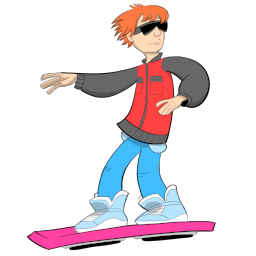
\includegraphics[width=1in]{images/HoverBoard-small.png}
	\end{wrapfigure}

	We denote the restriction on the hover board's movement by the vector
	$\mat{3 \\1}$. By this we mean that if
	the hover board traveled ``forward'' for one hour, it would move along a
	``diagonal'' path that would result in a displacement of 3 miles East and
	1 mile North of its starting location.
\end{minipage}

\begin{minipage}{\textwidth}
	\vspace{.5cm}
	\begin{wrapfigure}{l}{1in}
	\vspace{-.8cm}
	
\includegraphics[width=1in]{images/MagicCarpet-small.png}
	\end{wrapfigure}

	We denote the restriction on the magic carpet's movement by the vector
	$\mat{1 \\2 }$. By this we mean that if the
	magic carpet traveled ``forward'' for one hour, it would move along a
	``diagonal'' path that would result in a displacement of 1 mile East and
	2 miles North of its starting location.
\end{minipage}

\lfoot{\footnotesize Drawings by \url{@DavidsonJohnR} (twitter)}

\vspace{10mm}

% Scenario Section
\textbf{Scenario One: The Maiden Voyage}

Your Uncle Cramer suggests that your first adventure should be to go visit
the wise man, Old Man Gauss. Uncle Cramer tells you that Old Man Gauss
lives in a cabin that is 107 miles East and 64 miles North of your home.

\vspace{5mm}

\textbf{Task:}
\par
Investigate whether or not you can use the hover board and the magic
carpet to get to Gauss's cabin. If so, how? If it is not possible to
get to the cabin with these modes of transportation, why is that the case?

%\vspace{5mm}
% As a group, state and explain your answer(s) on the group whiteboard. Use
% the vector notation for each mode of transportation as part of your
% explanation and use a diagram or graphic to help illustrate your
% point(s).


\begin{lesson}
	\Title{Linear Combinations}

	\Heading{Textbook}
	Section 1.2

	\Heading{Objectives}
	\begin{itemize}
		\item Set up and solve vector equations $a\vec v+b\vec u=\vec w$. The solving
			method may be ad hoc.
		\item Use set notation and set operations/relations $\cup$, $\cap$, $\in$, $\subseteq$.
		\item Translate between set-builder notation and words in multiple ways.
	\end{itemize}

	\Heading{Motivation}
	We revisit questions about linear combinations more formally and generate a need for
	algebra. The algebra we do to solve vector equations will become algorithmic when
	we learn row reduction, but at the moment, any method is fine.

	\begin{annotation}
		\begin{notes}
			You will have a mix of MAT135/136 and MAT137 students.
			The MAT137 students will be doing logic and sets in their
			class. The MAT135 students won't. Make sure not to leave them
			behind!
		\end{notes}
	\end{annotation}
	As we talk about more complex objects, we need precise ways to talk about
	groups of vectors. I.e., we need sets and set-builder notation. This preview of set-builder
	notation will take some of difficulty away when we define span as a set of vectors.

	In this course we will be using formal and precise language. Part of this lesson
	is that there are multiple correct ways (and multiple incorrect ways) to use formal
	language. Gone are the days of ``there's only one right answer and it is 4''!

\end{lesson}


\section*{Task 1.2: The Magic Carpet Ride, Hide and Seek}
\addcontentsline{toc}{subsection}{Task 1.2: The Magic Carpet Ride, Hide and Seek}


\begin{annotation}
	\begin{goals}
		\Goal{Address an existential question involving vectors: ``Is it possible
		to find a linear combination that does\ldots?''}

		The goal of this problem is to
		\begin{itemize}
			\item Formalize geometric questions using the language of vectors.
			\item Find both geometric and algebraic arguments to support the same
				conclusion.
			\item Establish what a ``negative multiple'' of a vector should be.
		\end{itemize}
	\end{goals}
	\begin{notes}
		\begin{itemize}
			\item Both \emph{yes} and \emph{no} are valid answers to
				this question depending on whether you are allowed
				to go backwards. Establish that ``negative'' multiples of
				a vector mean traveling backwards along that vector.
			\item This problem can be solved with algebra by finding a formula
				for the coefficients for an arbitrary position or with geometry,
				with arguments eventually hinging on the fact that non-parallel
				lines do not intersect.
		\end{itemize}
	\end{notes}
\end{annotation}
You are a young traveler, leaving home for the first time. Your parents
want to help you on your journey, so just before your departure, they give
you two gifts. Specifically, they give you two forms of transportation:
a hover board and a magic carpet. Your parents inform you that both the
hover board and the magic carpet have restrictions in how they operate:



\begin{minipage}{\textwidth}
	\vspace{.5cm}
	\begin{wrapfigure}{l}{1in}
	\vspace{-.8cm}
	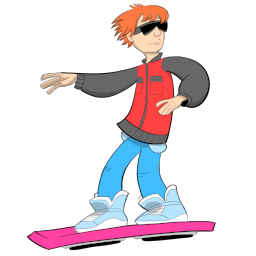
\includegraphics[width=1in]{images/HoverBoard-small.png}
	\end{wrapfigure}

	We denote the restriction on the hover board's movement by the vector
	$\mat{3 \\1}$. By this we mean that if
	the hover board traveled ``forward'' for one hour, it would move along a
	``diagonal'' path that would result in a displacement of 3 miles East and
	1 mile North of its starting location.
\end{minipage}

\begin{minipage}{\textwidth}
	\vspace{.5cm}
	\begin{wrapfigure}{l}{1in}
	\vspace{-.8cm}
	
\includegraphics[width=1in]{images/MagicCarpet-small.png}
	\end{wrapfigure}

	We denote the restriction on the magic carpet's movement by the vector
	$\mat{1 \\2 }$. By this we mean that if the
	magic carpet traveled ``forward'' for one hour, it would move along a
	``diagonal'' path that would result in a displacement of 1 mile East and
	2 miles North of its starting location.
	\vspace{1cm}
\end{minipage}



\textbf{Scenario Two: Hide-and-Seek}

Old Man Gauss wants to move to a cabin in a different location. You are
not sure whether Gauss is just trying to test your wits at finding him
or if he actually wants to hide somewhere that you can't visit him.

\vspace{5mm}

\textbf{Are there some locations that he can hide and you cannot reach him
with these two modes of transportation?}

Describe the places that you
can reach using a combination of the hover board and the magic carpet and
those you cannot. Specify these geometrically and algebraically. Include
a symbolic representation using vector notation. Also, include a convincing
argument supporting your answer.

%\vspace{5mm} \par \textbf{Use your
%group's whiteboard as a space to write out our work as your work together
%on this problem.}



\pagestyle{siefken}

\section*{Sets and Set Notation}
\vspace{-.5cm}

	\begin{definition}[Set]
		A \emph{set} is a (possibly infinite) collection of items
		and is notated with curly braces (for example, $\{1,2,3\}$ is
		the set containing the numbers 1, 2, and 3).  We call the items in
		a set \emph{elements}.

		If $X$ is a set and $a$ is an element of $X$, we may write $a\in X$,
		which is read ``$a$ is an element of $X$.''

		If $X$ is a set, a \emph{subset} $Y$ of $X$ (written $Y\subseteq X$)
		is a set such that every element of $Y$ is an element of $X$. Two sets are
		called \emph{equal} if they are subsets of each other (i.e., $X=Y$ if
		$X\subseteq Y$ and $Y\subseteq X$).

		We can define a subset using \emph{set-builder notation}.
		That is, if $X$ is a set, we can define the subset
		\[
			Y= \Set*{a\in X \given \text{some rule involving }a},
		\]
		which is read ``$Y$ is the set of $a$ in $X$ {\bf such that} some rule
		involving $a$ is true.''  If $X$ is intuitive, we may omit it and
		simply write $Y=\{a:\text{some rule involving }a\}$.  You may equivalently
		use ``$|$'' instead of ``$:$'', writing $Y=\{a\,|\,\text{some rule involving }a\}$.
	\end{definition}

	\begin{definition}
		Some common sets are
		\begin{itemize}
			\item[] $\N=\Set{\text{natural numbers}} = \Set{\text{non-negative whole numbers}}$.
			\item[] $\Z=\Set{\text{integers}} = \Set{\text{whole numbers, including negatives}}$.
			\item[] $\R=\Set{\text{real numbers}}$.
			\item[] $\R^n=\Set{\text{vectors in $n$-dimensional Euclidean space}}$.
		\end{itemize}
	\end{definition}


	\question
	\begin{annotation}
		\begin{goals}
			\Goal{Practice reading sets and set-builder notation.}

			The goal of this problem is to
			\begin{itemize}
				\item Become familiar with $\in$, $\subseteq$, and $=$ in
					the context of sets.
				\item Distinguish between $\in$ and $\subseteq$.
				\item Use quantifiers with sets.
			\end{itemize}
		\end{goals}

		\begin{notes}
			\begin{itemize}
				\item Most are easy up through (h).
				\item Make students ``fix'' (i) so it
					becomes true.
				\item (j) and (k) are an opportunity to use
					the definition of set equality. Students don't
					realize that $=$'s has a definition.
			\end{itemize}
		\end{notes}
	\end{annotation}
	\begin{parts}
		\item Which of the following statements are true?
		\begin{enumerate}
			\item $3\in\Set{1,2,3}$.
				\begin{solution}[inline]True\end{solution}
			\item $1.5\in\Set{1,2,3}$.
				\begin{solution}[inline]False\end{solution}
			\item $4\in\Set{1,2,3}$.
				\begin{solution}[inline]False\end{solution}
			\item ``b''$\in \Set{ x \given x\text{ is an English letter}}$.
				\begin{solution}[inline]True\end{solution}
			\item ``\`o''$\in \Set{x \given x\text{ is an English letter}}$.
				\begin{solution}[inline]False\end{solution}
			\item $\Set{1,2} \subseteq \Set{1,2,3}$.
				\begin{solution}[inline]True\end{solution}
			\item For some $a\in \Set{1,2,3}$, $a \geq 3$.
				\begin{solution}[inline]True\end{solution}
			\item For any $a\in \Set{1,2,3}$, $a\geq 3$.
				\begin{solution}[inline]False\end{solution}
			\item $1 \subseteq \Set{1,2,3}$.
				\begin{solution}[inline]False\end{solution}
			\item $\Set{1,2,3}=\Set{x\in\R \given 1\leq x\leq 3}$.
				\begin{solution}[inline]False\end{solution}
			\item $\Set{1,2,3}=\Set{x\in\Z \given 1\leq x\leq 3}$.
				\begin{solution}[inline]True\end{solution}
		\end{enumerate}
	\end{parts}

	\question
	\begin{annotation}
		\begin{goals}
			\Goal{Practice writing sets using set-builder notation.}

			The goal of this problem is to
			\begin{itemize}
				\item Express English descriptions using math notation.
				\item Recognize there is more than one correct way to
					write formal math.
				\item Preview vector form of a line.
			\end{itemize}
		\end{goals}

		\begin{notes}
			\begin{itemize}
				\item There are multiple correct ways to write
					each of these sets. It's a good opportunity
					to get man correct and incorrect sets up on the
					board for discussing.
				\item Don't worry about the geometry of $B$. That's coming
					in a later problem.
			\end{itemize}
		\end{notes}
	\end{annotation}
		Write the following in set-builder notation
	\begin{parts}
			\item The subset $A\subseteq \R$ of real numbers larger than $\sqrt{2}$.
				\begin{solution}
					$\Set*{x\in\R \given x>\sqrt{2}}$.
				\end{solution}
			\item The subset $B\subseteq \R^2$ of vectors whose first coordinate
			is twice the second.
				\begin{solution}
					$\Set*{\vec v\in\R^2\given \vec v=\mat{a\\b}\text{ with }a=2b}$
					or
					$\Set*{\vec v\in\R^2\given\vec v=\mat{2t\\t}\text{ for some }t\in \R}$\\
					or
					$\Set*{\mat{a\\b}\in\R^2\given a=2b}$.
				\end{solution}
	\end{parts}

	\begin{definition}[Unions \& Intersections]
		Two common set operations are \emph{unions} and \emph{intersections}.
		Let $X$ and $Y$ be sets.

		\hfill\begin{minipage}{\dimexpr\textwidth-3cm}
		\begin{itemize}
			\item[(union)] $X\cup Y = \Set{ a \given a\in X\text{ or }a\in Y}$.
			\item[(intersection)] $X\cap Y = \Set{ a \given a\in X\text{ and }a\in Y}$.
		\end{itemize}
		\end{minipage}
	\end{definition}

	\question
	\begin{annotation}
		\begin{goals}
			\Goal{Apply the definition of $\cup$ and $\cap$.}
		\end{goals}

		\begin{notes}
			\begin{itemize}
				\item It's not important to emphasize that $\cup$ and $\cap$ are binary
			operations but we ask for $X\cup Y\cup Z$ without parenthesis.
			Students won't worry if you don't bring it up.
				\item It won't be clear to them how to write the empty set.
					Some will write $\{\emptyset\}$. Make sure this comes out.
			\end{itemize}
		\end{notes}
	\end{annotation}
	Let $X=\Set{1,2,3}$ and $Y=\Set{2,3,4,5}$ and $Z=\Set{4,5,6}$.  Compute
	\begin{parts}
		\item $X\cup Y$ \begin{solution}[inline]$\Set{1,2,3,4,5}$\end{solution}
		\item $X\cap Y$ \begin{solution}[inline]$\Set{2,3}$\end{solution}
		\item $X\cup Y\cup Z$ \begin{solution}[inline]$\Set{1,2,3,4,5,6}$\end{solution}
		\item $X\cap Y\cap Z$ \begin{solution}[inline]$\emptyset=\Set{}$\end{solution}
	\end{parts}


\begin{lesson}
	\Title{Visualizing Sets, Formal Language of Linear Combinations}

	\Heading{Textbook}
	Section 1.2

	\Heading{Objectives}
	\begin{itemize}
		\item Draw pictures of formally-described subsets of $\R^2$.
		\item Graphically represent $\cup$ and $\cap$ for subsets of $\R^2$.
		\item Graphically represent linear combinations and then come up with
			algebraic arguments to support graphical intuition.
	\end{itemize}

	\Heading{Motivation}

	We want to build a bridge between the formal language of linear combinations
	and set-builder notation and geometric intuition. Where as last time
	the focus was on formal language, this time the focus is on linking geometry
	to formal descriptions.


\end{lesson}

	\question
	\begin{annotation}
		\begin{goals}
			\Goal{Visualize sets of vectors.}

			The goal of this problem is to
			\begin{itemize}
				\item Apply set-builder notation in the context of vectors.
				\item Distinguish between ``for all'' and ``for some''
					in set builder notation.
				\item Practice unions and intersections.
				\item Practice thinking about set equality.
			\end{itemize}
		\end{goals}

		\begin{notes}
			\begin{itemize}
				\item 1--3 will be easy.
				\item Have a discussion about when you
					should draw vectors as arrows
					vs\mbox{.} as points.
				\item 4 gets at a subtle point that will come up again
					when we define span.
				\item Many will miss 7. Writing a proof for this is
					good practice.
			\end{itemize}
		\end{notes}
	\end{annotation}
	Draw the following subsets of $\R^2$.
	\begin{parts}
		\item $V=\Set*{\vec x\in\R^2 \given \vec x=\mat{0\\t}\text{ for some }t\in\R}$.
		\item $H=\Set*{\vec x\in\R^2 \given \vec x=\mat{t\\0}\text{ for some }t\in\R}$.
		\item $D=\Set*{\vec x\in\R^2 \given \vec x=t\mat{1\\1}\text{ for some }t\in\R}$.
		\begin{solution}
	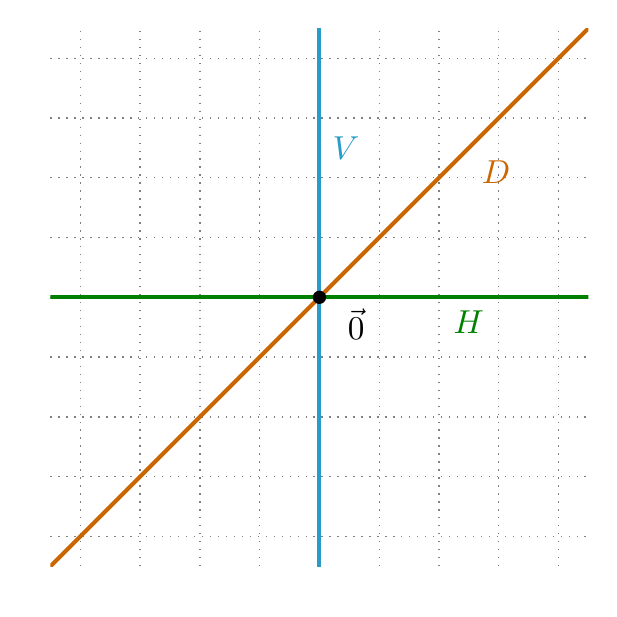
\begin{tikzpicture}[scale=1.2, >=latex]
    \begin{axis}[scale=1,
		    axis equal image,
		    axis line style={draw=none},
		    tick style={draw=none},
		    yticklabels={,,},
		    xticklabels={,,},
		 xmin=-4.5,
		 xmax=4.5,
		 ymin=-4.5,
		 ymax=4.5,
		 major grid style={dotted, gray},
                 xtick={-10,-9,...,10},
                 ytick={-10,-9,...,10},
                 grid=both,
		 anchor=origin]

	    \draw[Green, very thick] (-5,0) -- (5,0) node[near end, below] {$H$};
	    \draw[cyan!80!black, very thick] (0,-5) -- (0,5) node[near end, right] {$V$};
	    \draw[orange!80!black, very thick] (-5,-5) -- (5,5) node[near end, below right] {$D$};

	    \fill[fill=black] (0,0) circle[radius=2pt] node[below right, xshift=5pt] {\color{black}$\vec 0$};
    \end{axis}
\end{tikzpicture}
		\end{solution}
		\item $N=\Set*{\vec x\in\R^2 \given \vec x=t\mat{1\\1}\text{ for all }t\in\R}$.
				\begin{solution}[inline]
			$N=\Set{}$.
		\end{solution}

		\item $V\cup H$.
			\begin{solution}[inline]
			$V\cup H$ looks like a ``$+$'' going through the origin.
		\end{solution}
		\item $V\cap H$.
			\begin{solution}[inline]
				$V\cap H=\Set{\vec 0}$ is just the origin.
		\end{solution}
		\item Does $V\cup H=\R^2$?
			\begin{solution}
				No. $V\cup H$ does not contain $\mat{1\\1}$ while $\R^2$ does contain
				$\mat{1\\1}$.
			\end{solution}
	\end{parts}

\section*{Vector Combinations}
	\vspace{-1em}

	\begin{definition}[Linear Combination]
		A \emph{linear combination} of the vectors $\vec v_1,\vec v_2,\ldots,\vec v_n$ is
		a vector
		\[
			\vec w = \alpha_1\vec v_1+\alpha_2\vec v_2+\cdots+\alpha_n\vec v_n.
		\]
		The scalars $\alpha_1,\alpha_2,\ldots,\alpha_n$ are called the \emph{coefficients} of the linear combination.
	\end{definition}

	\question
	\label{ProbSkewBasis}
	\begin{annotation}
		\begin{goals}
			\Goal{Practice linear combinations.}

			The goal of this problem is to
			\begin{itemize}
				\item Practice using the formal term \emph{linear combination}.
				\item Foreshadow span.
			\end{itemize}
		\end{goals}

		\begin{notes}
			\begin{itemize}
				\item In 2, the question should arise: ``Is $3\vec v_1$
					a linear combination of $\vec v_1$ \emph{and}
					$\vec v_2$?'' Address this.
				\item Refer to the magic carpet ride for 5. You don't
					need to do a full proof.
			\end{itemize}
		\end{notes}
	\end{annotation}
	Let $\vec v_1=\mat{1\\1}$, $\vec v_2=\mat{1\\-1}$, and $\vec w=2\vec v_1+\vec v_2$.
	\begin{parts}
		\item Write $\vec w$ as a column vector. When $\vec w$ is written as a
			linear combination of $\vec v_1$ and $\vec v_2$, what are the
			coefficients of $\vec v_1$ and $\vec v_2$?
			\begin{solution}
				$\vec w=\mat{3\\2}$; the coefficients are $(2,1)$.
			\end{solution}
		\item Is $\mat{3\\3}$ a linear combination of $\vec v_1$ and $\vec v_2$?
			\begin{solution}[inline]
				Yes. $\mat{3\\3}=3\vec v_1+0\vec v_2$.
			\end{solution}

		\item Is $\mat{0\\0}$ a linear combination of $\vec v_1$ and $\vec v_2$?
			\begin{solution}[inline]
				Yes. $\vec 0=0\vec v_1+0\vec v_2$.
			\end{solution}
		\item Is $\mat{4\\0}$ a linear combination of $\vec v_1$ and $\vec v_2$?
			\begin{solution}[inline]
				Yes. $\mat{4\\0}=2\vec v_1+2\vec v_2$.
			\end{solution}
		\item Can you find a vector in $\R^2$ that isn't a linear combination of
		$\vec v_1$ and $\vec v_2$?
			\begin{solution}
				No. $\mat{1\\0}=\tfrac{1}{2}\vec v_1+\tfrac{1}{2}\vec v_2$ and
				$\mat{0\\1}=\tfrac{1}{2}\vec v_1-\tfrac{1}{2}\vec v_2$.
				Therefore
				\[
					\mat{a\\b}
					= a\mat{1\\0}+b\mat{0\\1}
					= a(\tfrac{1}{2}\vec v_1+\tfrac{1}{2}\vec v_2)
						+b(\tfrac{1}{2}\vec v_1-\tfrac{1}{2}\vec v_2)
					=(\tfrac{a+b}{2})\vec v_1+(\tfrac{a-b}{2})\vec v_2.
				\]
				Therefore any vector in $\R^2$ can be written as linear combinations
				of $\vec v_1$ and $\vec v_2$.
			\end{solution}
		\item Can you find a vector in $\R^2$ that isn't a linear combination of
			$\vec v_1$?
			\begin{solution}
				Yes. All linear combinations of $\vec v_1$ have equal $x$ and
				$y$ coordinates, therefore $\vec w=\mat{2\\1}$ is not a linear
				combination of $\vec v_1$.
			\end{solution}
	\end{parts}


	\question
	\begin{annotation}
		\begin{goals}
			\Goal{Practice formal writing.}
		\end{goals}

		\begin{notes}
			\begin{itemize}
				\item Make everyone \emph{write}. They will think
					they can do it, but they will find it hard if
					they try.
			\end{itemize}
		\end{notes}
	\end{annotation}
	Recall the \emph{Magic Carpet Ride} task where the hover board could
	travel in the direction $\vec h=\mat{3\\1}$ and the magic carpet could
	move in the direction $\vec m=\mat{1\\2}$.
	\begin{parts}
		\item Rephrase the sentence \emph{``Gauss can be reached using just the
			magic carpet and the hover board''} using formal mathematical
			language.
			\begin{solution}
				Gauss's location can be written as a linear combination of
				$\vec m$ and $\vec h$.
			\end{solution}
		\item Rephrase the sentence \emph{``There is nowhere Gauss can hide
			where he is inaccessible by magic carpet and hover board''} using
			formal mathematical language.
			\begin{solution}
				Every vector in $\R^2$ can be written as a linear combination
				of $\vec m$ and	$\vec h$.
			\end{solution}
		\item Rephrase the sentence \emph{``$\R^2$ is the set of all linear
			combinations of $\vec h$ and $\vec m$''} using formal mathematical
			language.
			\begin{solution}
				$\R^2=\Set{\vec v\given \vec v=t\vec m+s\vec h\text{ for some }t,s\in \R}$.
			\end{solution}
	\end{parts}

\begin{lesson}
	\Title{Restricted Linear Combinations, Lines}

	\Heading{Textbook} Section 1.2

	\Heading{Objectives}
	\begin{itemize}
		\item Read and digest a new definition.

		\item Use pictures to explore a new concept.

		\item Convert from an equation-representation of a line to a set-representation.
	\end{itemize}

	\Heading{Motivation} Part of doing math in the world is reading and understanding
	other people's definitions. Most students will not have heard of non-negative
	linear combinations or convex linear combinations. This is a chance for them
	to read and try to understand these formal definitions. They will need to
	draw pictures to get an intuition about what these concepts mean.

	These concepts are useful in their own right, and in particular, convex linear
	combinations can be used to describe line segments. Adding these definitions
	to a student's toolbox serves the goal of \emph{being able to describe
	the world with mathematics}.

	To that end, we start working with lines. Lines are something students have
	used since grade school, but they worked with them in $y=mx+b$ form which
	is only applicable in $\R^{2}$. We want to convert this representation
	into vector form and set-based descriptions which apply to all
	dimensions.

\end{lesson}

	\displayonlynewpage
	\begin{definition}[Non-negative \& Convex Linear Combinations]
		The linear combination $\vec w=\alpha_1\vec v_1+\alpha_2\vec v_2+\cdots+\alpha_n\vec v_n$ is
		called a \emph{non-negative} linear combination of $\vec v_1,\vec v_2,\ldots,\vec v_n$ if
		$\alpha_1,\alpha_2,\ldots,\alpha_n\geq 0$.

		If $\alpha_1,\alpha_2,\ldots,\alpha_n\geq 0$
		and $\alpha_1+\alpha_2+\cdots+\alpha_n=1$, then $\vec w$ is called a \emph{convex} linear combination
	of  $\vec v_1,\vec v_2,\ldots,\vec v_n$.
	\end{definition}

	\question
	\begin{annotation}
		\begin{goals}
			\Goal{Geometric meaning of \emph{non-negative} and \emph{convex}
			linear
			combinations.}

			The goal of this problem is to
			\begin{itemize}
				\item Read and apply the definition of non-negative and convex
					linear combinations.
				\item Gain geometric intuition for non-negative and convex linear
					combinations.
				\item Learn how to describe line segments using
					convex linear combinations.
			\end{itemize}
		\end{goals}

		\begin{notes}
			\begin{itemize}
				\item This question is about reading and applying;
					emphasize that before they start.
				\item The geometry won't be obvious. Ask them to \emph{draw} specific
					linear combinations (e.g., $(1/2,1/2)$) to get an idea.
				\item They know $\vec a$ and $\vec b$ span all vectors from problem \ref{ProbSkewBasis}.
				\item In part 1, they will forget $\vec a$ and $\vec b$ are linear combinations of themselves.
				\item Part 2 (b) highlights a degeneracy that will come up again when discussing linear independence and dependence. Explain how the 
					picture for non-negative linear combinations
					almost always looks one way, but this case is an exception.
			\end{itemize}
		\end{notes}
	\end{annotation}
	Let
	\[
		\vec a=\mat{1\\1} \qquad \vec b=\mat{-1\\1}\qquad \vec c=\mat{0\\1}\qquad\vec d=\mat{0\\2}\qquad\vec e=\mat{-1\\-1}.
	\]
	\begin{parts}
		\item Out of $\vec a$, $\vec b$, $\vec c$, $\vec d$, and $\vec e$, which
			vectors are
			\begin{enumerate}
				\item linear combinations of $\vec a$ and $\vec b$?
				\begin{solution}[inline]
					All of them, since any vector in $\R^2$ can be written as a linear combination
					of $\vec a$ and $\vec b$.
				\end{solution}

				\item non-negative linear combinations of $\vec a$ and $\vec b$?
				\begin{solution}[inline]
					$\vec a$, $\vec b$, $\vec c$, $\vec d$.
				\end{solution}

				\item convex linear combinations of $\vec a$ and $\vec b$?
				\begin{solution}[inline]
					$\vec a$, $\vec b$, $\vec c$.
				\end{solution}
			\end{enumerate}

		\item If possible, find two vectors $\vec u$ and $\vec v$ so that
			\begin{enumerate}
				\item $\vec a$ and $\vec c$ are non-negative linear combinations
					of $\vec u$ and $\vec v$ but $\vec b$ is not.
				\begin{solution}
					Let $\vec u=\vec a$ and $\vec v=\vec c$.
				\end{solution}

				\item $\vec a$ and $\vec e$ are non-negative linear combinations
					of $\vec u$ and $\vec v$.
				\begin{solution}
					Let $\vec u=\vec a$ and $\vec v=\vec e$.
				\end{solution}

				\item $\vec a$ and $\vec b$ are non-negative linear combinations
					of $\vec u$ and $\vec v$ but $\vec d$ is not.
				\begin{solution}
					Impossible. If $\vec a$ and $\vec b$ are non-negative
					linear combinations of $\vec u$ and $\vec v$, then every non-negative
					linear combination of $\vec a$ and $\vec b$ is also a non-negative
					linear combination of $\vec u$ and $\vec v$. And, we already concluded that
					$\vec d$ is a non-negative linear combination of $\vec a$ and $\vec b$.
				\end{solution}

				\item $\vec a$, $\vec c$, and $\vec d$ are convex linear
					combinations of $\vec u$ and $\vec v$.
				\begin{solution}
					Impossible. Convex linear combinations all lie on the same line segment,
					but $\vec a$, $\vec c$, and $\vec d$ are not collinear.
				\end{solution}
			\end{enumerate}Otherwise, explain why it's not possible.
	\end{parts}

	\displayonlynewpage
\section*{Lines and Planes}

	\question
	\begin{annotation}
		\begin{goals}
			\Goal{Link prior knowledge to new notation/concepts.}

			The goal of this problem is to
			\begin{itemize}
				\item Convert between $y=mx+b$ form of a line and
					the set-builder definition of the same line.
				\item Think about lines in terms of vectors rather
					than equations.
			\end{itemize}
		\end{goals}

		\begin{notes}
			\begin{itemize}
				\item This question is foreshadowing for vector form of a line.
				\item In part 3, some will draw $\vec d$ from the origin and
					some will draw it on the line. Both are fine, but make
					sure they understand that $\vec d\notin L$ by the end of
					part 4.
			\end{itemize}
		\end{notes}
	\end{annotation}
	Let $L$ be the set of points $(x,y)\in\R^2$ such that $y=2x+1$.
	\begin{parts}
		\item Describe $L$ using set-builder notation.
			\begin{solution}
				$\Set*{\vec v\in\R^2 \given \vec v=\matc{t\\2t+1}\text{ for some } t\in\R}$\\
				or
				$\Set*{\mat{x\\y}\in\R^2 \given y=2x+1}$
				or
				$\Set*{\matc{t\\2t+1}\in\R^2 \given t\in\R}$
			\end{solution}
		\item Draw $L$ as a subset of $\R^2$.
		\item Add the vectors $\vec a=\mat{-1\\-1}$, $\vec b=\mat{1\\3}$ and
			$\vec d=\vec b-\vec a$ to your drawing.
			\begin{solution}
				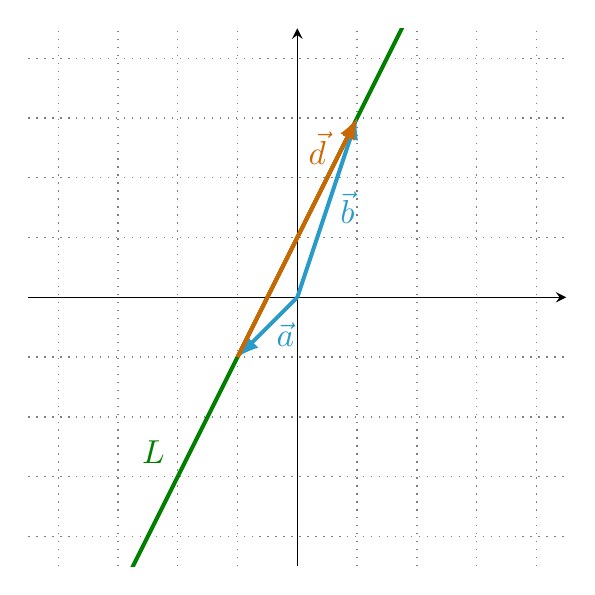
\begin{tikzpicture}[scale=1.2, >=latex]
			    \begin{axis}[scale=1,
					    axis equal image,
					    axis lines=middle,
					    axis line style = {black},
					    tick style={draw=none},
					    yticklabels={,,},
					    xticklabels={,,},
					 xmin=-4.5,
					 xmax=4.5,
					 ymin=-4.5,
					 ymax=4.5,
					 major grid style={dotted, gray},
					 xtick={-10,-9,...,10},
					 ytick={-10,-9,...,10},
					 grid=both,
					 anchor=origin]

				    \draw[Green, very thick] (-5,-9) -- (5,11) node[pos=.3, above left] {$L$};
				    \draw[cyan!80!black, very thick, ->] (0,0) -- (-1,-1) node[pos=.2, below] {$\vec a$};
				    \draw[cyan!80!black, very thick, ->] (0,0) -- (1,3) node[pos=.5, right] {$\vec b$};
				    \draw[orange!80!black, very thick, ->] (-1,-1) -- (1,3) node[near end, above, xshift=-3pt] {$\vec d$};

			    \end{axis}
				\end{tikzpicture}
			\end{solution}
		\item Is $\vec d\in L$? Explain.
			\begin{solution}
				No. $\vec d=\mat{2\\4}$ and so its entries don't satisfy $y=2x+1$.
			\end{solution}
		\item For which $t\in\R$ is it true that $\vec a+t\vec d\in L$? Explain using your picture.
			\begin{solution}
				$\vec a +t\vec d\in L$ for any $t\in \R$. We can see this because if we start at the
				vector $\vec a$ and the displace by $t\vec d$, we will always be on the line $L$.
			\end{solution}
	\end{parts}




\end{document}
